%%%%%%%%%%%%%%%%%%%%%%%%%%%%%%%%%%%%%%%%%%%%%%%%%%%%%%%%%%%%%%%%%%%%%%%
%% $Id: report.tex,v 1.5 2005/02/09 21:06:42 lindstrm Exp $
%%%%%%%%%%%%%%%%%%%%%%%%%%%%%%%%%%%%%%%%%%%%%%%%%%%%%%%%%%%%%%%%%%%%%%%
%% costhesis usage example
%% modified and added to by GQMJr
%%%%%%%%%%%%%%%%%%%%%%%%%%%%%%%%%%%%%%%%%%%%%%%%%%%%%%%%%%%%%%%%%%%%%%%
%
% The costhesis package accepts the following options
%
%   Document types:
%     msc               - Master Thesis
%     bsc		- Kandidate Thesis
%
%   Layout options:
%
%   Other options:
%     blank             - Removes pagenumbers and headers from empty pages
%     blankmsg          - Prints a message of intent on empty pages
%     scheader          - Typeset headers in SMALL CAPS shape (default)
%     slheader          - Typeset headers in slanted shape 
%
%
%
%

\documentclass[12pt,a4paper,twoside,openright]{book}
%%\documentclass[12pt,a4paper,twoside,openright]{memoir}

\usepackage[msc,blankmsg]{costhesis}
%\usepackage[T1]{fontenc}
%%\usepackage{pslatex}
\renewcommand{\rmdefault}{ptm} 
\usepackage{mathptmx}
\usepackage[scaled=.90]{helvet}
\usepackage{courier}
%
\usepackage{bookmark}
\usepackage{caption}
\usepackage{subcaption}

%%----------------------------------------------------------------------------
%%   pcap2tex stuff
%%----------------------------------------------------------------------------
 \usepackage[dvipsnames*,svgnames]{xcolor} %% For extended colors
 \usepackage{tikz}
 \usetikzlibrary{arrows,decorations.pathmorphing,backgrounds,fit,positioning,calc,shapes}
 \usepackage{pgfmath}	% --math engine
%%----------------------------------------------------------------------------
%\usepackage[latin1]{inputenc}
\usepackage[utf8]{inputenc} % inputenc allows the user to input accented characters directly from the keyboard
\usepackage[swedish,english]{babel}
\usepackage{rotating}		 %% For text rotating
\usepackage{array}			 %% For table wrapping
\usepackage{graphicx}	 %% Support for images
\usepackage{float}			 %% Suppor for more flexible floating box positioning
\usepackage{color}           %% Support for colour 
\usepackage{mdwlist}
\usepackage{setspace}    %% For fine-grained control over line spacing
\usepackage{listings}		%% For source code listing
\usepackage{bytefield}    %% For packet drawings
\usepackage{tabularx}		%% For simple table stretching
\usepackage{multirow}	%% Support for multirow colums in tables
\usepackage{dcolumn}	%% Support for decimal point alignment in tables
\usepackage{url}	%% Support for breaking URLs
\usepackage{epstopdf}
\usepackage[perpage,para,symbol]{footmisc} %% use symbols to
                                %% ``number'' footnotes and reset
                                %% which symbol is used first on each
                                %% page

%%\usepackage{pygmentize}  %% required to use minted -- see python-pygments - Pygments is a Syntax Highlighting Package written in Python
%%\usepackage{minted}		%% For source code highlighting

\usepackage{hyperref}		
\usepackage[all]{hypcap}	 %% Prevents an issue related to
                                %% hyperref and caption linking
\usepackage[backend=biber, sorting=none]{biblatex}
\addbibresource{biblio.bib}

%% setup hyperref to use the darkblue color on links
\hypersetup{colorlinks,breaklinks,
            linkcolor=darkblue,urlcolor=darkblue,
            anchorcolor=darkblue,citecolor=darkblue}


%% Some definitions of used colors
\definecolor{darkblue}{rgb}{0.0,0.0,0.3} %% define a color called darkblue
\definecolor{darkred}{rgb}{0.4,0.0,0.0}
\definecolor{red}{rgb}{0.7,0.0,0.0}
\definecolor{lightgrey}{rgb}{0.8,0.8,0.8} 
\definecolor{grey}{rgb}{0.6,0.6,0.6}
\definecolor{darkgrey}{rgb}{0.4,0.4,0.4}
%% Reduce hyphenation as much as possible
\hyphenpenalty=15000 
\tolerance=1000

%% useful redefinitions to use with tables
\newcommand{\rr}{\raggedright} %% raggedright command redefinition
\newcommand{\rl}{\raggedleft} %% raggedleft command redefinition
\newcommand{\tn}{\tabularnewline} %% tabularnewline command redefinition

%% definition of new command for bytefield package
\newcommand{\colorbitbox}[3]{%
	\rlap{\bitbox{#2}{\color{#1}\rule{\width}{\height}}}%
	\bitbox{#2}{#3}}

%% command to ease switching to red color text
\newcommand{\red}{\color{red}}
%%redefinition of paragraph command to insert a breakline after it
\makeatletter
\renewcommand\paragraph{\@startsection{paragraph}{4}{\z@}%
  {-3.25ex\@plus -1ex \@minus -.2ex}%
  {1.5ex \@plus .2ex}%
  {\normalfont\normalsize\bfseries}}
\makeatother

%%redefinition of subparagraph command to insert a breakline after it
\makeatletter
\renewcommand\subparagraph{\@startsection{subparagraph}{5}{\z@}%
  {-3.25ex\@plus -1ex \@minus -.2ex}%
  {1.5ex \@plus .2ex}%
  {\normalfont\normalsize\bfseries}}
\makeatother

\setcounter{tocdepth}{3}	%% 3 depth levels in TOC
\setcounter{secnumdepth}{5} %% 3 sectioning levels. WARNING: command \mainmatter resets this field to its default value!!!
%%%%%%%%%%%%%%%%%%%%%%%%%%%%%%%%%%%%%%%%%%%%%%%%%%%%%%%%%%%%%%%%%%%%
%% End of preamble
%%%%%%%%%%%%%%%%%%%%%%%%%%%%%%%%%%%%%%%%%%%%%%%%%%%%%%%%%%%%%%%%%%%%

\iauthor{Antonios Kouzoupis}
\ititle{High performance shared state schedulers}
\isubtitle{}
\idate{2016}{July}{1}
\examinername{Associate professor Jim Dowling}
\supervisorname{Professor Seif Haridi}
\kthlogo{resources/images/KTH_logo.eps}
\itrita{YYYY}{NN}

\setlength{\headheight}{15pt}
\begin{document}

\frontmatter
\selectlanguage{english}
\begin{abstract}
\label{sec:abstract}
\setcounter{page}{1}

Large organizations and research institutes store a huge volume of data nowadays.
In order to gain any valuable insights distributed processing frameworks over a
cluster of computers are needed. Apache Hadoop is the prominent framework for distributed
storage and data processing. At SICS Swedish ICT we are building Hops, a new distribution
of Apache Hadoop relying on a distributed, highly available MySQL
Cluster NDB to improve performance. Hops-YARN is the resource management framework of Hops
which introduces distributed resource management, load balancing the
tracking of resources in a cluster. In Hops-YARN we make heavy usage of the
back-end database storing all the resource manager metadata and
incoming RPCs to provide high fault tolerance and very short recovery
time.

This project aims in optimizing the mechanisms used for persisting
metadata in NDB both in terms of transactional commit time but also
in terms of pre-processing them. Under no condition should the in-memory RM
state diverge from the state stored in NDB. With these goals in mind
several solutions were examined that improved the performance of the
system, making Hops-YARN comparable to Apache YARN with the extra benefits
of high-fault tolerance and short recovery time. The solutions
proposed in this thesis project enhance the pure commit time of a
transaction to the MySQL Cluster and the pre-processing and parallelism
of our Transaction Manager. The results indicate that the performance
of Hops increased dramatically, utilizing more resources on a cluster
with thousands of machines. Increasing the cluster utilization by a
few percentages can save organizations a big amount of money.


\end{abstract}
%%\clearpage
\selectlanguage{swedish}
%%\chapter*{Sammanfattning}
\begin{abstract}
\label{sec:swedish_abstract}

IETF xxxx Arbetsgruppen har definierat

\end{abstract}

\selectlanguage{english}
\begin{acknowledgements}

I would like to thank my examiner Jim Dowling for his invaluable
insights and crucial guidelines throughout this project and my
supervisor at KTH Seif Haridi. Also, I would like to express my
sincere gratitude to my supervisor at SICS Gautier Berthou for his
endless support, guidance and patience. He and his expertise was
the source of motivation and really helpful regardless the problem.

\end{acknowledgements}

\selectlanguage{english}
\tableofcontents

\listoffigures

\listoftables

%% add a list of listing if and listings are used
\lstlistoflistings

% \begin{notations}
% \end{notations}

\renewcommand\abbreviationsname{List of Acronyms and Abbreviations}
\begin{abbreviations}
\label{list-of-acronyms-and-abbreviations}

\begin{basedescript}{\desclabelstyle{\pushlabel}\desclabelwidth{10em}}
\item[YARN] Yet Another Resource Negotiator
  \cite{Vavilapalli:2013:AHY:2523616.2523633}
\item[HDFS] Hadoop Distributed File System \cite{hdfs}
\item[RM] Resource Manager
\item[NM] Node Manager
\item[AM] Application Master
\item[RT] Resource Tracker
\item[HA] High availability
\item[NDB] Network Database
\end{basedescript}

\end{abbreviations}

\mainmatter
\setcounter{secnumdepth}{5} 
\chapter{Introduction}
\label{chap:introduction}
In the last years, the storage capacity of hard disk drives has
increased dramatically while at the same time their price has
decreased. Even though solid-state drives are still quite expensive,
big enterprises may benefit from the throughput they provide. This
trend of ``cheap'' storage solutions has led companies and research
institutes to store a volume of data that has never been stored
before. In 2014 Facebook was processing 600 TB daily
\footnote{https://code.facebook.com/posts/229861827208629/scaling-the-facebook-data-warehouse-to-300-pb/}
while according to rough estimates
\footnote{https://what-if.xkcd.com/63/} around 15 exabytes are stored
in Google's datacenters.

Another interesting area that is already generating a huge volume of
raw data is the DNA sequencing. According to \cite{10.1371/journal.pbio.1002195} the Sequence
Read Archive maintained by the United States National Institutes of Health
National Center for Biotechnology Information already contains more
than 3.6 petabytes of raw sequence data for a wide variety of samples
including microbial genomes, plant and animal genomes and human
genomes. As we can see in Figure \ref{fig:intro_genomics_growth} the
need for storage capacity will exceed the order of PetaBytes by the
year 2025.

\begin{figure}
\centering
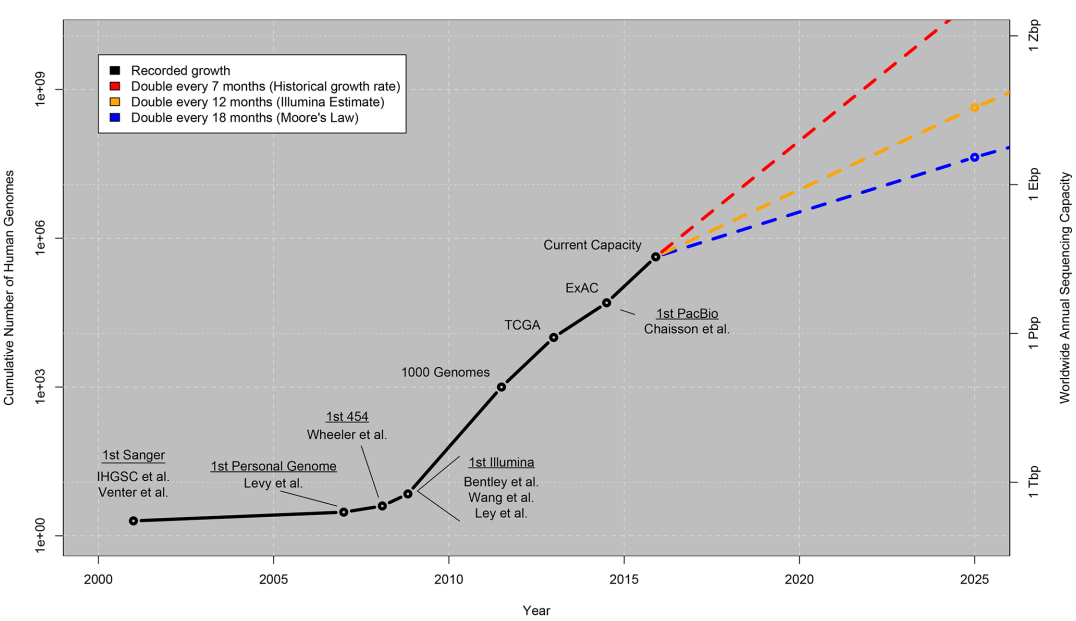
\includegraphics[scale=0.5]{resources/images/Introduction/genomics_growth.png}
\caption{Growth of DNA sequencing \cite{10.1371/journal.pbio.1002195}}
\label{fig:intro_genomics_growth}
\end{figure}

It is clear by now that these volumes need a paradigm shift
from the traditional way we store and analyze data. It is not possible
anymore to store them in a single machine. We need to employ a
distributed system to harness the power of those data and extract
valuable results within a reasonal time frame. On top of that we have
to take under consideration that hardware will fail for various
reasons. A minimum requirement would be not to lose our data, so we
should keep them in several replicas. Going one step further, we would
like our analyzing jobs to continue running even though one machine failed. These
jobs usually take hours to complete, so re-running them is not the
best approach.


%% Longer problem statement
%% General introduction to the area
\section{Problem description}
\label{sec:problem_description}
As it is already mentioned, datasets now days are in the order of
petabytes and exabytes. Distributed file systems like GFS
\cite{Ghemawat:2003:GFS:1165389.945450}, 
GlusterFS \cite{glusterfs}, HDFS \cite{Shvachko:2010:HDF:1913798.1914427} etc come to extend
the traditional file systems located in a single machine. Storing the
datasets is one half of the problem though. The second part is
managing the computational resources on a cluster. A cluster consists
of several physical machines, sometimes thousands of them, and each
machine has numerous CPUs and RAM modules. Users of the cluster issue
their jobs with certain CPU and RAM requirements, as well as the files
which they want to access. On a very high level abstraction there is
an entity which has knowledge of the available resources and should
schedule the jobs accordingly. The view of the cluster from the
\emph{scheduler} perspective is updated frequently with the new
cluster utilization.

This project is a work on Hops \cite{hops} platform
and more specifically on Hops-YARN, which is a modified version of
Apache Hadoop YARN \cite{Vavilapalli:2013:AHY:2523616.2523633}. In YARN the
entity which is responsible for keeping an updated version of the
cluster utilization and scheduling tasks is the \emph{Resource
Manager} (RM). The view of RM regarding the available resources on the
cluster is updated frequently (by default 1 second) by a heartbeating
mechanism. On each machine of the cluster there is the \emph{Node
Manager} (NM) which periodically sends updates for the machine
usage. Users issue their application requests to the RM which then
allocates a container to create the \emph{Application Master}
(AM). The AM service is working independently and is responsible to
keep track of the application health and any further resource
requests. AM periodically heartbeats the RM (by default 1 second)
stating its health, the application progress or any resource
increase/decrease.

An aware reader should have already noticed that RM is a crucial part
of the Hadoop platform for managing resources. Not only it is vital
for the progress of the system but also it can become a
bottleneck and a single point of failure. Until recently, Spotify was
provisioning a cluster of 1300
Hadoop nodes \footnote{http://conferences.oreilly.com/strata/big-data-conference-ca-2015/public/schedule/detail/38595}. Every single node has to heartbeat the RM every
second. On top of that for every single application launched, the AM
service should also heartbeat the RM. This produces a considerable
amount of load on the RM side which has to handle all those heartbeats
and also make scheduling decisions.

In Hops in order to improve performance and HA of the RM we have introduced an
in-memory distributed MySQL database which stores all the necessary
metadata. One great feature of Hops-YARN is that the
\emph{ResourceTrackerService} (RT) of the RM is distributed into multiple
nodes in the cluster. That service is responsible for receiving and handling
heartbeats from the NMs. That way each instance handles only a portion of the total NM
heartbeats. The updated metadata are then stored into the database and
are streamed to the RM to update its view of the cluster. By load
balancing the ResourceTrackerService we have increased the performance
of the system while decreasing the load of the master RM which can
perform the rest of the operations without the load of handling every
single heartbeat.

Another equally important feature of Hops-YARN is that RM stores
every event received and any scheduling decision into the MySQL
cluster. That makes our solution highly available with minimum
failover period. When a RM instance fails it re-builds the view of the
cluster by reading the latest state from the database. More details on
the architecture of both YARN and Hops-YARN will be given in Chapter
\ref{chap:background} and \ref{chap:implementation}.

\section{Problem statement}
\label{sec:problem_statement}
Even with high
throughput, low latency network between the RM/RT and the database, it
still takes more time than in-memory operations. Especially in cases
where RM operations need more than one round-trip to the database, the
difference in performance is noticeable.

A great advantage of using a relational database is the support of
foreign key constraints. The information that we store is semantically
related. In a SQL schema that is directly translated to foreign key
constraints. A trivial example is information regarding the containers
running on node and information regarding the node itself. Clearly, we
should never run into a situation where we try to persist a container
running on a node without having information about the node at
all. Moreover, foreign key constraints work the other way around. By
removing the information about a node from the database we want the
information about running containers on that node to be purged
too. Such constraints, although they seem tempting to use, pose a
great performance degradation as we will show later in this thesis. Particularly when we aim for millions
of operations per second, the use of foreign key constraints should be
limited and very well designed.

The transaction state manager of Hops should try to commit
various states in parallel as much as possible but on the other hand
ensure the order of two colliding states. For example there should
never be the case where two states change information about the same
node in the cluster and yet be committed in parallel. Similarly, two
states that change information in the database about different
entities should be committed in parallel.

The distributed MySQL cluster database is a central building block in our
architecture. A slow commit and process time will result in less events being
streamed and handled by the RM, directly affecting the cluster
utilization and the view of the cluster from the RM perspective.
A slow commit time will decrease the
rate of handled events while increase the rate of queued events that
are waiting to be handled. Our goal is to be able to scale up to 10000 NMs
with multiple RTs. With the current mechanism this is not possible due
to delays both in the transaction manager mechanism and in the commit
time.

\section{Goals, Benefits, Ethics and Sustainability}
\label{sec:goals_ethics}
This is going to be my goals, benefits, ethics and sustainability section...

\section{Structure of this thesis}
\label{sec:thesis_structure}
\section{Structure of this thesis}
\label{sec:thesis_structure}
This is the structure of this thesis

\chapter{Background}
\label{chap:background}
This chapter will give the reader the necessary background knowledge
in order for this work to be understandable. First, it will go through
Apache Hadoop, a distributed storage and processing framework. We will
give some brief introduction to Hadoop file system (HDFS), then we
will dive into the
resource manager (YARN) and in what way HopsYarn extend the Apache
YARN project. Later we will introduce a distributed, highly-available,
highly-redundant relational database, MySQL Cluster (NDB) and finally
we will give some insights on the different types of resource managing
systems.

In Figure \ref{fig:back_hpc_arch_overview} we can see a high level
overview of the architecture in HPC. Storage nodes are machines with very high disk capacity and bare
minimum processing power. Their main usage is to store data that are
going to be processed and analyzed in the future. The second building
block of the architecture is the Computing nodes. These machines have
no storage capabilities but they are equiped with the state of the art
processing units and a lot of RAM. Those modules communicate most
probably with a high throughput, low latency network. The most common
industry standard for interconnecting nodes in HPC is InfiniBand
\cite{infiniband} that it can
reach 30 Gb/s in each direction and sub-microsecond latency. Users
issue their jobs to the Head node which is responsible for transfering
the requested datasets from the Storage nodes to the Computing nodes,
monitor the tasks and finally return the result to the end user.

\begin{figure}
\centering
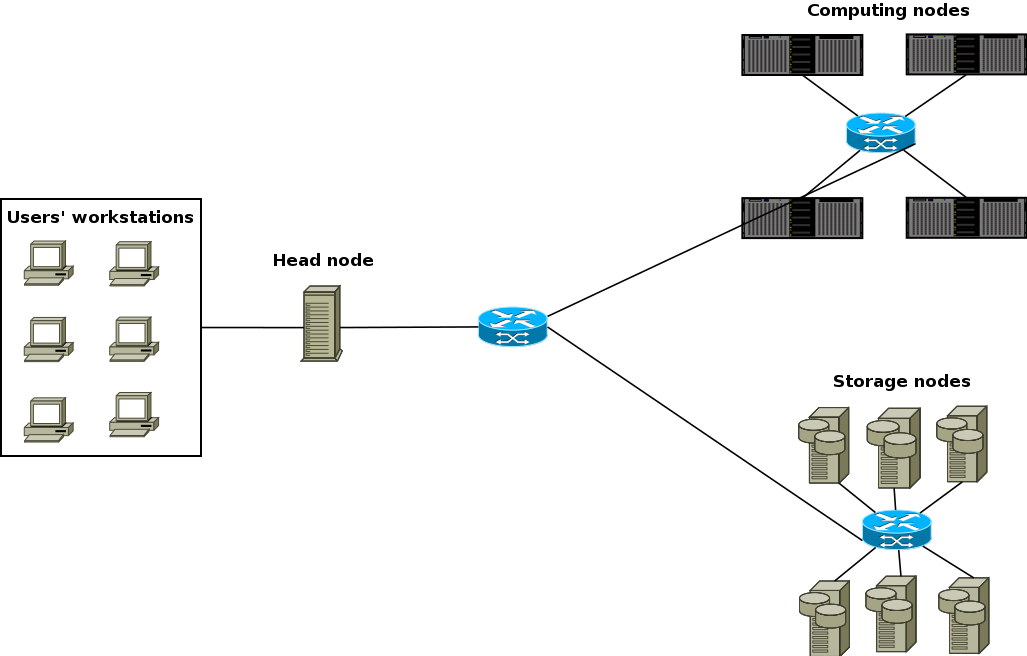
\includegraphics[scale=0.35]{resources/images/Background/hpc_arch_overview.png}
\label{fig:back_hpc_arch_overview}
\caption{HPC high level architecture}
\end{figure}

In 2003 Google published a paper describing GoogleFS (GFS)
\cite{Ghemawat:2003:GFS:1165389.945450}, a proprietary distributed
file system. It was designed to run on large clusters of commodity
hardware, that are doomed to fail at some time. That was the main
motivation that drove GFS to be fault-tolerant and
highly-available. Apache HDFS is the open-source implementation of GFS
and it will be analyzed in Section \ref{ssec:hdfs}. In 2004 Google
published MapReduce \cite{Dean:2004:MSD:1251254.1251264}, a breakthrough programming model which exploited the locality
awareness of GFS and changed the way we process very big
datasets. MapReduce was later implemented for Hadoop and paved the way
for YARN, the current resource manager and scheduler 
which will be analyzed in Section \ref{ssec:yarn}.


\section{Hadoop}
\label{sec:hadoop}
Apache Hadoop is an open-source framework for distributed storage of
large datasets and processing across clusters of computers. It was
created in 2006 after the release of GFS
\cite{Ghemawat:2003:GFS:1165389.945450} and MapReduce
\cite{Dean:2004:MSD:1251254.1251264} papers from Google. The core part
of Hadoop comprises of its distributed file system -- HDFS, and the
job scheduling, resource management framework -- YARN.

The attribute that makes the biggest difference in Hadoop and similar
projects is that of data locality awareness. In contrast to the HPC
architecture, we do not distinguish anymore between processing and
storage nodes. All nodes in a cluster perform both roles. Datasets are
split into blocks of data. To provide fault tolerance each block is
replicated in several nodes in the cluster. Moreover, there is a
central authority which keeps track of the nodes each block is stored.

With that feature in mind, we do not move datasets anymore to the
computing nodes but the executable of our job to the nodes where our
data reside. When the processing of the individual blocks is done, we
gather the result. That is a great paradigm shift from the traditional way
of processing big datasets. A high level overview of the Hadoop
architecture is depicted in Figure
\ref{fig:hadoop_arch_overview}. Datasets are split into blocks and
are stored in the nodes of cluster, both the original and the
replicas. When a user submits a job, the workflow manager will copy
the job to the appropriate nodes, which in parallel will execute
it. Finally, the workflow manager will gather the individual results,
aggregate them and return the final result to the client.

\begin{figure}
\centering
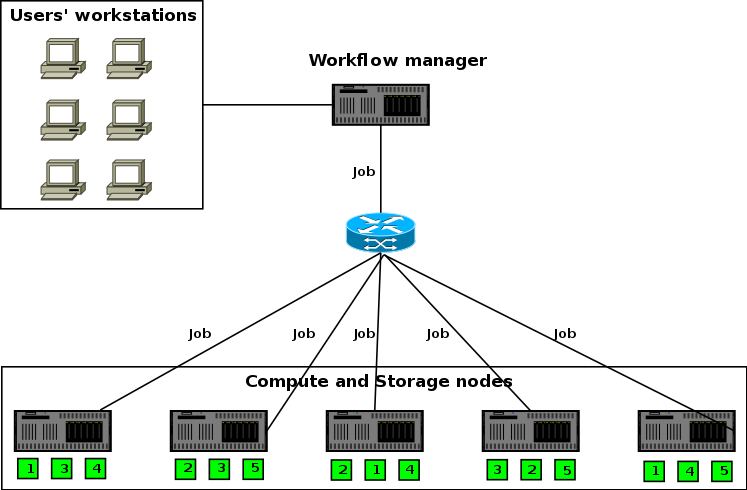
\includegraphics[scale=0.5]{resources/images/Background/hadoop_arch_overview.png}
\label{fig:hadoop_arch_overview}
\caption{Hadoop high level architecture}
\end{figure}

\section{HDFS}
\label{sec:hdfs}
As this project is focused on the resource management framework, I will
not give a detailed description of the Hadoop Distributed File
System. Yet, I will go through some basic concepts that will make the
reader understand better the overall architecture of Hadoop.

HDFS is the distributed file system of Hadoop platform. It is designed
with the assumption that hardware failure is the norm and not an
exception making it highly fault-tolerant. Also, it is designed to run
on commodity, heterogeneous, low-cost hardware making the setup and provisioning of
a cluster cheaper than in HPC. HDFS has two main entities, the NameNode
(NN) and the DataNode (DN) and its architecture is depicted in Figure
\ref{fig:hadoop_hdfs}.

\begin{figure}
\centering
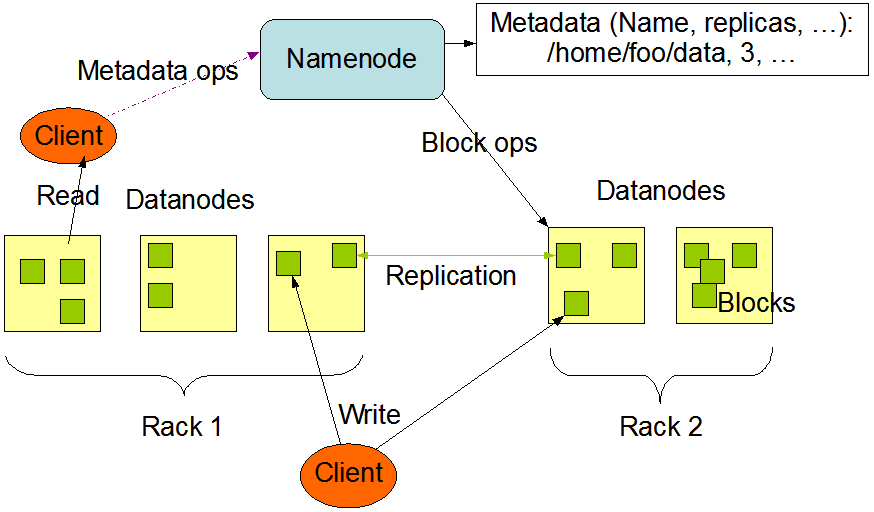
\includegraphics[scale=0.5]{resources/images/Background/hdfs_arch.png}
\caption{HDFS architecture \cite{hdfs}}
\label{fig:hadoop_hdfs}
\end{figure}

\subsection{NameNode}
\label{ssec:nn}

An HDFS cluster consists of a single active NN that is responsible for the
file system metadata, the blocks replication and the health
status of the DNs.

HDFS exposes to a user a file system similar to POSIX, in terms that
the structure is hierarchical, there are the same file permissions 
and a subset of POSIX operations. A user through the NN can open,
close, read, delete a file as in any file system. The NN uses a transaction
log, the \emph{EditLog}, that persists to the local file system any
operation that is done to the HDFS namespace. For example if a file is
renamed then a record is added to the EditLog, or if the replication
factor for a file is changed.

As HDFS was designed to run on commodity
hardware it should be able to handle machine failures. Internally, a
file is split in a number of blocks. Typically each block is 128 MB,
except from the last one and are stored
in the DNs. HDFS replicates the blocks to other machines--DNs
according to a configurable replication factor and replication policy.
If the DN that holds a specific block has crashed, then that block is read from
another replica in another DN.
The NN keeps a file in its local file system with the entire namespace
and the mapping of blocks to DNs, called \emph{FsImage}. Upon
recovery, the NN reads the FsImage and applies any operation that is
logged in the EditLog. That way it can recover from a scheduled
maintenance reboot or from a crash.

The NN periodically receives heartbeats from the DNs that have dual
purpose. The first one is to maintain a health status for the DNs. If
the NN misses a heartbeat from a DN, then it marks that DN as
dead. From that point no blocks will be further assigned to that DN
and NN will start migrating all the blocks that reside in that DN to
others. The second reason of receiving heartbeats is to maintain an
updated view of the \emph{BlockMap}, the mapping of blocks to
DNs. When a DN sends a heartbeat to the NN, it piggybacks a list with
the blocks that it currently stores. That way, the BlockMap in the NN
is kept up-to-date with the blocks that are stored in every DN.

\subsection{DataNode}
\label{ssec:dn}

The DN is the slave entity in the HDFS master/slave architecture as depicted in
Figure \ref{fig:hadoop_hdfs} and the actual storage of blocks. Upon a
client request to store a file in HDFS, the NN instructs it (the
client) which DNs to contact to store the individual file block. The
same procedure is followed when a client requests to read a file. The
NN returns a list with DNs that store the blocks forming the whole
file. The client then contacts each and every DN, fetching the
corresponding blocks.

A DN periodically heartbeats to NN. As I have explained in Section
\ref{ssec:nn}, the heartbeat contains a list of blocks, that the DN
issued the heartbeat stores, so that the NN maintains a map of file
blocks and DataNodes. Also, the heartbeat signifies that the DN is
alive and can be used for storage and retrieval of blocks. Heartbeats
also carry information regarding the status of the DN such as total
storage capacity, storage in use etc. These metrics are taken
consideration by the NN when assigning blocks to DN.

The DataNode also perform various operations as instructed by the
NN. These instructions are sent to the DN via the heartbeat
mechanism as a reply to the heartbeat sent by the DN. Such operations
might be creation, deletion or replication of a block. The block
replication is done according to the replication strategy. A common
strategy for placing replicas with a replication factor of three, is
to place the first replica in the same node as the client runs, the
second in another node in a different rack (off-rack) and the third
one in the same rack as the second but in a different node. Adjusting
the replication factor and the replication policy can greatly affect
the write and read performance of the HDFS cluster and should be
carefully tweaked.


\section{Data computation and Resource management}
\label{sec:resource_mgm}
Something general about MapReduce and YARN resource management

\subsection{MapReduce}
\label{ssec:mapreduce}
After the world wide web explosion at the ending of 1990's, Google has
emerged as one of the most significant web searching companies.
The novelty of Google was PageRank \cite{ilprints361}, an
algorithm counting the number of outgoing links of a webpage to determine its
importance. In order to apply the PageRank algorithm and form the
Google search results, first the webpage has to be scraped and
indexed. As of 2004 the raw size of the documents that had been
collected was more than 20 terabytes
\cite{Dean:2004:MSD:1251254.1251264}. Although the engineers at Google
have distributed and parallelized the algorithm, there were more tasks
that other teams have parallelized in a different way making it
difficult to maintain such a diverse codebase. That led them in 2004
to publish a paper about MapReduce, a generic framework to write distributed
applications that hide all the complexity of fault-tolerance, locality
awareness, load balancing etc.

MapReduce programming model borrows two very common functions from
functional programming, \emph{Map} and \emph{Reduce}. The \emph{Map}
function takes as input key/value pairs and produces as output a set
of key/value pairs as well. The \emph{Map} function is written by the
user and varies depending on the use case.

The \emph{Reduce} function, takes as input the
intermediate key/value pairs produced by \emph{Map} and merge them
together producing a smaller set of values. The \emph{Reduce} function
and the way it will merge the intermediate pairs is also provided by
the user.

A trivial example of the MapReduce programming model is that of
counting the occurrences of words in a text. The \emph{Map} function
takes as input a list of all the words in the text and emits a tuple
in the form \texttt{(word,1)}, where \texttt{word} is every word
parsed. The result of the \emph{Map} function is passed to the
\emph{Reduce} function which adds the value of the tuples with the
same key, in that case is the word. The result will be a list of
tuples where the key is all the words parsed from the text and the
value would be the occurrences of the word in the text.

Google provided a framework which took advantage of the locality
awareness of the already existing GFS and the MapReduce programming
paradigm. The execution overview of MapReduce is depicted in Figure
\ref{fig:mapreduce_execution_overview}. We can identify two entities
in MapReduce architecture, the \emph{Master} and the \emph{Workers}.

\begin{figure}
\centering
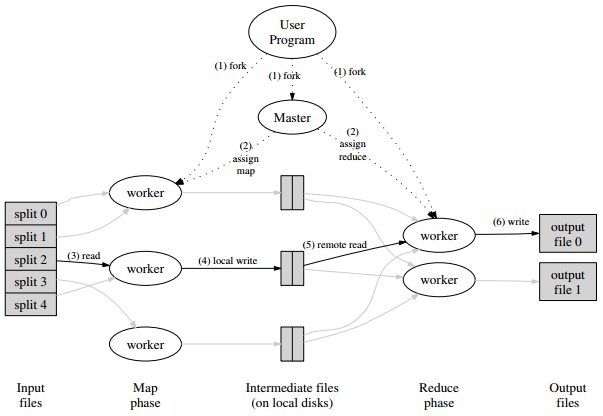
\includegraphics[scale=0.8]{resources/images/Background/mapreduce_exec_overview.png}
\label{fig:mapreduce_execution_overview}
\caption{MapReduce execution overview \cite{Dean:2004:MSD:1251254.1251264}}
\end{figure}

The \emph{Master} has the role of the coordinator that pushes the jobs
to the worker machines. It keeps track of the status of jobs in the
workers, informs other workers for the intermediate files produced
during the Map phase and pings the workers to verify their liveness.

The \emph{Workers} reside at the same physical hardware as the GFS
nodes to take advantage of the data locality. They are divided into
\emph{mappers}, which execute the Map function and \emph{reducers},
which perform the reduce phase as instructed. Workers are
pre-configured with available map or reduce slots depending on their
CPU or RAM.

At the very beginning, a user submits a job to Master. Master forks
the submitted job and is responsible to schedule the forks on workers
that $(a)$ have available map/reduce slots and $(b)$ have the
requested datasets stored locally. Upon the scheduling is done, the
Map phase begins in the mappers. They read the datasets from the local
hard drive and perform the Map function. Master periodically pings the
mappers to get informed about the status of the job and the health of
the node itself. When a mapper node completes its task, it writes the
intermediate key/value pairs to the local file system and informs the
Master node. The Master node in turn, notifies the reducer nodes that
an intermediate result is available at a specific node, where the
latter reads it (the result) remotely and perform the reduce
function. Finally, when all the reducers have completed the Reduce
phase, the Master notifies the user program.

\subsubsection{MapReduce Fault Tolerance}
Primary concern of the engineers was the fact
that machines will eventually fail. MapReduce will run on a cluster of
thousands of machines so the probability of a failed machine would be
higher. For that reason they equipped MapReduce with a heartbeating
mechanism in order to be able to handle such situations.
The Master periodically pings the workers. The workers should respond back
within a predefined timeout before they are declared dead. When a node
that performs the Map phase is declared dead, then the job that was
running at that node is set to \emph{idle} and is rescheduled on
another node. Similarly, when a map job has finished, since the
intermediate result is written to the local hard drive, the job has to
be rescheduled in a different machine. When a reducer node has failed
and the job is still in \emph{running} state, then it is set back in
\emph{idle} state and assigned to another node. In case of a completed
Reduce phase, the result is stored in the global file system, GFS in
that case. So, even with a failed reducer machine, the result will
still be available and the job should not be rescheduled.

While a Worker failure does not greatly affect the MapReduce job, it
is not the same case with a Master failure. If a machine that is a
Master node fails, then the whole MapReduce job is canceled and the
client is informed so that it can retry later on. ``However, given
that there is only a single master, its failure is unlikely;''
\cite{Dean:2004:MSD:1251254.1251264}.

\subsubsection{Limitations}
MapReduce facilitated engineers to ``easily'' write parallel data
processing applications by hiding all the complexity of a distributed
system. It provided some sort of fault tolerance and it was generic
enough to fit in various domains.

MapReduce and Hadoop over the years has become the industry standard
for processing and storing big volumes of data. After some period of
heavy usage it became clear that, although the platform itself suited
the needs for distributed, reliable storage and cluster management,
there were some limitations that had to be addressed. The two key
shortcomings were regarding the tight coupling of a programming model
with the resource management infrastructure and the centralized
handling of jobs \cite{Vavilapalli:2013:AHY:2523616.2523633, 6680946}.

A user who wanted to write an application for MapReduce framework,
all it had to do was to provide implementation for the two
first-order functions \emph{Map} and \emph{Reduce}. This static
map-reduce pipeline is very limiting though, as every job should have exactly one
Map function followed by an optional Reduce function. That workflow is
not suitable for large scale computations, such as machine learning
programs that require multiple iterations over a dataset. That means
that multiple individual MapReduce jobs had to be scheduled while the
frequent write of data in disk or in a distributed file system would
impose a considerable latency. A common pattern/misuse
\cite{Vavilapalli:2013:AHY:2523616.2523633} was to submit jobs with a
map phase only that spawned alternative frameworks or even web
servers. The scheduler had no semantics about the job except that they
were map jobs with a consequence in the cluster utilization, creating
deadlocks and a general instability to the system. The second drawback
of MapReduce and Hadoop 1.x was the centralized job handling and
monitoring of their flow. The Master or the \emph{JobTracker} should
monitor every single job, receiving liveness heartbeats, resource
requests etc. The is a heavy workload for a single machine that drove
to major scalability issues.

These two crucial limitations of MapReduce led to a total re-design of
Hadoop. Since Hadoop 2.0 there is a resource management module, YARN --
\emph{Yet Another Resource Negotiator} which will be analyzed in
section \ref{ssec:yarn} and MapReduce is just another application
running on a cluster of physical machines.

\subsection{YARN}
\label{ssec:yarn}
Considering the limitations outlined in section
\ref{sssec:mapreduce_limitations}, Vinod Kumar Vavilapalli et
al. presented YARN \cite{Vavilapalli:2013:AHY:2523616.2523633} the new
resource management layer that was adopted in Hadoop 2.0. The new
Hadoop stack now is depicted in Figure \ref{fig:yarn_hadoop1_hadoop2_arch} where YARN is the
cluster resource management module and MapReduce is one out of plenty
applications running on top of YARN. This architectural transformation
paved the way for a wide variety of frameworks like
Apache Spark \cite{apache_spark}, Apache Flink \cite{apache_flink},
Apache Pig \cite{apache_pig}, etc to run on the
Hadoop platform like any other YARN application.

\begin{figure}
\centering
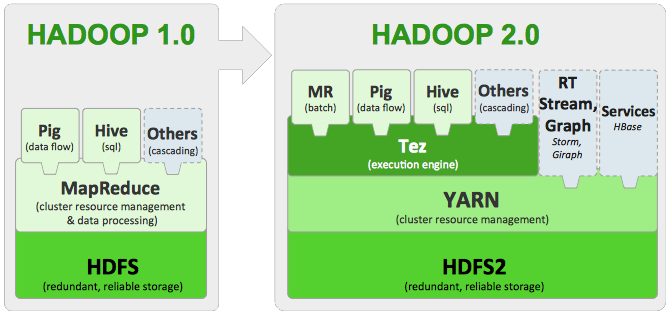
\includegraphics[scale=0.6]{resources/images/Background/hadoop1_hadoop2_arch.png}
\label{fig:yarn_hadoop1_hadoop2_arch}
\caption{Hadoop 2.0 stack \cite{hortonworks_hadoop_stack}}
\end{figure}

The new architecture of Hadoop 2.x separates the resource management
functions from the programming model. It delegates the
intra-application communication and the tracking of the execution flow
to per-job components. That unlocks great performance improvements,
improves scalability and enables a wide variety of frameworks to share
the cluster resources in a very gentle way.

YARN uses three main components to provide a scalable and fault
tolerant resource management platform. The first component is the
\emph{ResourceManager} (RM), a per-cluster daemon that tracks resource
usage and node liveness and schedules jobs on the cluster. The second
component is a per-node \emph{NodeManager} (NM) which is responsible
for monitoring resource availability on the specific node, reporting
faults to RM and managing container life-cycle. Finally, there is the
\emph{ApplicationMaster} (AM) which coordinates the logical plan of a
single job, manages the physical resources offered by the RM and
tracks the execution of the job. A high level overview of YARN
architecture is described in Figure \ref{fig:yarn_arch_overview}. RM
has a global view of the cluster and provides the scheduling
functionality, while the per-job AM manages the dynamic resource
requests and the workflow of the tasks. Containers that are allocated
by the RM are locally managed by the NM in each node in the cluster.

\begin{figure}
\centering
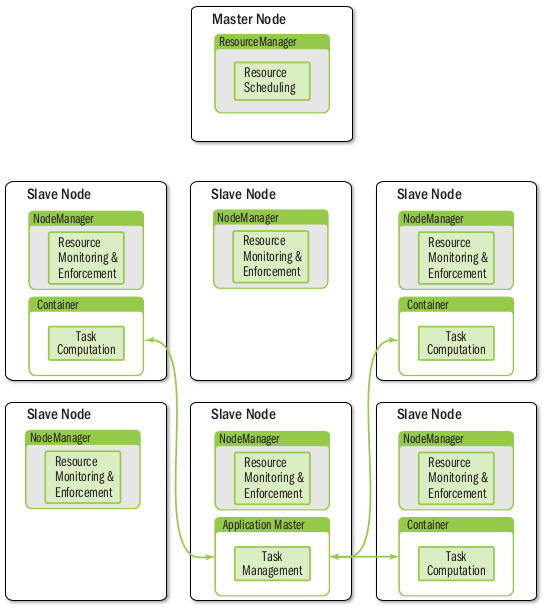
\includegraphics[scale=0.5]{resources/images/Background/yarn_arch_overview.png}
\label{fig:yarn_arch_overview}
\caption{YARN architecture overview \cite{Murthy:2014:AHY:2636998}}
\end{figure}

\subsubsection{ResourceManager}
\label{sssec:rm}
In YARN the RM acts as the central authority for allocating resources
in the cluster. It works closely with the per-node NodeManager getting
an updated view of the cluster by the heartbeats received. The RM
itself allocates generic resources in the cluster in the form of
\emph{containers} that have specific CPU and RAM requirements. Those
resource requests are piggybacked in the heartbeats issued by every AM.
As RM is completely unaware about the job execution plan,
it is up to the AM to make local optimizations and assign the
resources accordingly. RM internally consists of several modules but
the three most important are the \emph{ApplicationMasterService}, the
\emph{ResourceTrackerService} and the \emph{Yarn Scheduler} as shown
in Figure \ref{fig:yarn_RM_components}.

\begin{figure}
\centering
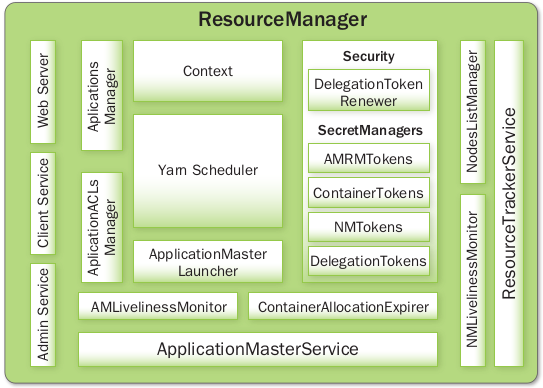
\includegraphics[scale=0.6]{resources/images/Background/RM_components.png}
\label{fig:yarn_RM_components}
\caption{ResourceManager components \cite{Murthy:2014:AHY:2636998}}
\end{figure}

The \emph{ApplicationMasterService} is responsible for receiving and
handling heartbeats from the AMs that are launched in the
cluster. Heartbeats are designed to be as compact as possible, still
not excluding any vital information. For that reason, Google Protocol
Buffers \cite{proto_buf} are used for every communication among YARN
components. Protocol Buffers is a language-neutral, platform-neutral
mechanism for efficiently serializing data. The heartbeat mechanism
serves both as a scalable way for the RM and AM to communicate, but
also for the RM to track the liveness of AMs. \emph{ResourceRequests}
contain information such as the resources per container in terms of
virtual cores and memory, the number of containers, locality
preferences and priority of requests. The scheduler then tracks,
updates and satisfies these requests with available resources in the
cluster. The RM builds the view of the cluster with the available
resources from the information it receives from the NMs. The scheduler
tries to match the locality constraints as much as possible and
responds back to AM with the allocated containers along with
credentials that grant access to them. The RM also keeps track of the
AM health through the heartbeats received. The component that handle
the liveness property of every AM is the \emph{AMLivenessMonitor}. In
case of a missed heartbeat, that particular AM is deemed dead and
is expired by the RM. All the containers that were allocated for
that AM are marked as dead and the RM reschedules the same application
(ApplicationMaster) on a new container.

As I have previously mentioned, the RM builds its view of the cluster
by the information that NMs send to it. The
\emph{ResourceTrackerService} component is responsible for handling such RPCs
and forwarding them to the appropriate modules. Before a new node in the
cluster is able to execute YARN jobs, it should first register itself
with the RM through the ResourceTrackerService and exchange some
security tokens. A heartbeat mechanism is also used in this place to
ensure the liveness of NMs and to receive updated information about
the available resources in the physical machine. The newly received
information about the available resources on that node is forwarded to the YARN
scheduler so it can make scheduling decisions. Also, a received
heartbeat is forwarded to the \emph{NMLivelinessMonitor} module which
keeps track of the health of NMs. If RM has not received any heartbeat
from a NM after a configurable timeout, then it is deemed dead and is
expired. All the containers that were currently running on that node
are also marked as dead and an event is sent to the scheduling module
not to schedule any job on that node. When the node restarts, it
registers again with the RM and it makes itself available for
scheduling again.

At the core of RM is the \emph{YarnScheduler} that is responsible of
making scheduling decisions based on the available resources on the
cluster and the resource requests issued by the AMs. Currently the
resource requirements of an AM are limited to the number of virtual
cores and to the amount of memory a container should
have. YarnScheduler is a pluggable module and at the time of writing
there are three different options. The first and original option is
the \emph{FIFO Scheduler} where jobs are served in a simple
first-in-first-out order with no sense of priorities. The second
scheduling policy is the \emph{Capacity Scheduler}
\cite{capacity_scheduler} developed by Yahoo! Capacity Scheduler
is primarily built for large clusters with resources that are shared
among different units in the same organization. There are different
queues serving jobs for various units while guaranteeing some minimum
capacity for each queue. Any excess capacity can be temporarily
allocated to other queues and a job with high priority will be executed
before any other job with lower priority. If a job cannot be scheduled
in its respective queue due to lack of resources and that queue is
below its fair share, then jobs in other queues can be preempted. Last
but not least is the \emph{Fair Scheduler} \cite{fair_scheduler}
developed by Facebook. In Fair Scheduler every application belongs to
a queue, by default the ``default'' queue. The basic idea is that
containers are allocated to the application with the fewer resources
assigned within the queue, providing a uniform distribution of the
available cluster resources in the long run. There can be multiple
queue with support for priorities, minimum and maximum shares and FIFO
ordering within the queue. Similar to Capacity Scheduler, Fair Scheduler
also has support for preemption of containers that are already
assigned. Currently the default scheduler for Hadoop is the Capacity Scheduler.

\subsubsection{ApplicationMaster}
\label{sssec:am}
Upon a successful submission of an application to RM, the latter
creates a special container in a node called
\emph{ApplicationMaster}. AM is a per-application process that
coordinates the execution plan of the application, negotiates
resources with the RM and monitors the assigned containers. AM
periodically heartbeats RM, default value is 10 minutes, to prove it
is alive and to dynamically request more resources or release
some. When AM is launched, it will compute the necessary requirements
and locality preferences, encode them and through the heartbeat
mechanism send them to RM. RM depending on the scheduling decisions it
has made it might respond back with any empty response or with
\emph{container leases} on different nodes. AM will contact the
respective NodeManagers, present them the leases and the NM will
create the containers. Afterwards, it (AM) is responsible to monitor the liveness
of the containers or implement any recovery functions. An overview of
the workflow explained above is illustrated in Figure \ref{fig:yarn_am_rm_interaction}.

\begin{figure}
\centering
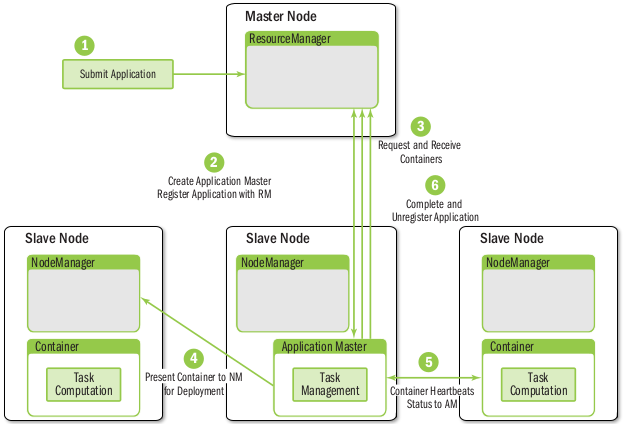
\includegraphics[scale=0.6]{resources/images/Background/AM_RM_interaction.png}
\label{fig:yarn_am_rm_interaction}
\caption{ApplicationMaster interaction \cite{Murthy:2014:AHY:2636998}}
\end{figure}

Since a key requirement for YARN was to decouple the programming model
from the resource management, AM is not tightly connected to YARN.
Writing an ApplicationMaster process is not an easy task but Hadoop
offers some APIs to avoid the complexity of low-level protocols.
Users can write their own ApplicationMaster
process fitting particular needs of making local optimizations with
the containers allocated by the RM, monitoring the containers,
define the recovery procedures when a container dies or capture the
exit status of a finished task. That opened the road for a plethora
of applications to run on Hadoop such as Apache Spark
\cite{apache_spark}, Apache Flink \cite{apache_flink}, Apache Hadoop
MapReduce \cite{apache_hadoop} etc.

\subsubsection{NodeManager}
\label{sssec:nm}
The \emph{NodeManager} is the ``worker'' daemon that runs on every
physical node of a Hadoop cluster. It is responsible for monitoring
the health of the physical hardware, authenticating the container
leases, preparing, monitoring and tearing down the container and
providing a set of services to the application.

When a node joins a cluster, the NM should register with the
RM. It will present the total amount of virtual cores and memory
available in this machine, some security tokens required to
authenticate the container leases, some communication ports etc. From
that point NM should periodically heartbeat the RM, default value is 1
second, proving that is still alive and keeping the RM up-to-date with
its status. NM regularly runs some monitoring scripts for the
health of the machine and the status is sent to RM. As a response it
might get back a list of container leases or some instructions such as
node decommission because of unhealthy node or to kill some
containers. In case of a missed heartbeat, the RM declares the NM as
dead, excludes that node from its pool of resources and informs all
running AMs about the failed NM. AM is responsible to react to such a
failure and possibly ask resources from RM to redo the work done in
the failed node.

Each container in YARN comes along with a \emph{container launch
  context} (CLC). The CLC contains information specific to the
application that is about to run such as environment variables,
dependencies stored in HDFS or on-line, security tokens, commands that
actually spawn the application etc. Once the NM has validated the
container lease with the security tokens provided, it should
initialize the container by fetching the requested dependencies,
setting the variables and of course run the commands specified by the
CLC. At the end of the container life-cycle or if the container dies
or if RM instructs NM to kill a container, NM should garbage collect
any dependency fetched during initialization and not used any
longer by other containers in that node. For the whole duration of a
container's life-cycle, NM monitors its utilization. If a container's
usage exceeds its assigned, then the NM signals the container to be
killed so that it does not disrupt the work of other containers
sharing the same physical machine. 

Finally, NM provides some services to the containers such as log
aggregation that will upload anything written to \texttt{stdout} or \texttt{stderr} to
HDFS when the application finishes. NM also provides a set of
auxiliary, pluggable services that are used by some applications. For
example, in MapReduce the intermediate output of the Map phase should
not be garbage collected after the container has finished. The
service will flag these data to be persisted even after the container
has gracefully exit.

\subsubsection{YARN fault tolerance \& HA}
\label{sssec:yarn_ha}
So far we have gone through some key points of the resource management
platform of Hadoop. RM is the central authority that makes scheduling
decisions and carries all the burden of monitoring both the AMs and
the NMs. Although from the beginning Hadoop was designed to run on
commodity hardware where machine failures are the norm
\cite{doi:10.2200/S00516ED2V01Y201306CAC024, Dean:2013:TS:2408776.2408794}, a
ResourceManager failure would drove the whole cluster
useless. Moreover, after a RM restart, it had to kill all the
containers running on the cluster including the ApplicationMasters and
launch new instances of them. Since RM is not responsible for the
recovery of the applications AMs had to start over the tasks, unless if
they had some recovery policy. Hadoop 2.4 introduced some kind of recovery mechanism that would
recover some application metadata and re-submit only the non-finished
applications in a way invisible to the user. As of Hadoop 2.6 RM
restart has further improved. The rest of this section will briefly
explain the recovery and HA mechanism of the RM.

To recover from a failure, RM needs to
store some state in a persistent storage. Currently there is support
for three alternatives. The first one is to use the Apache ZooKeeper
\cite{Hunt:2010:ZWC:1855840.1855851}, a service that provides highly reliable
distributed coordination, naming, storing and group membership
services. The second alternative is LevelDB \cite{google_leveldb},
a light-weight key-value store and finally the local file system or
HDFS. The default state store is the file system, local or HDFS, although
if a requirement of our cluster is also HA, then Apache ZooKeeper is
the preferred one. To begin with, RM stores some application metadata to
the persistent storage solution. These metadata include the
application submission context, the final status of the application,
diagnostics of the application and some security related
tokens. Moreover, when the RM restarts it will ask from all the NMs in
the cluster to re-sync and send back information about all the
containers that are currently running. Using that information it can
recover the whole state of the scheduler such as resource requests,
queues' usage etc. That way RM does not need to kill and kick-off again all
the running applications, just instruct the respective AMs to re-sync
with it.

Even with the aforementioned mechanism RM is a single point of
failure. In case of an RM crash, the cluster would be essentially useless until
the RM restarts and recover. This period, depending on the number of
nodes on the cluster, the number of applications running and the
policies to detect a dead machine, might take quite a long time. As of
Hadoop 2.4 there is a High Availability feature for the RM, using an
Active/Standby architecture and a ZooKeeper instance to coordinate
the RM nodes. ZooKeeper
ensures that at any point of time there is only one Active node that
performs all the scheduling decisions and monitoring operations. In case of a crash, a new leader is elected
from the Standby pool and is promoted to Active. The transition from
Standby to Active can be done either manually through the administration
CLI or automatically where ZooKeeper will detect the crashed node and
elect a new leader. The new Active RM will build the current state
from the state stored in ZooKeeper. AMs and NMs will keep contacting
the crashed, previously Active, RM until they realize it is dead. Then
they will contact the next RM in their configuration list until they
hit the currently Active node in a round-robin fashion.

\section{MySQL Cluster}
\label{sec:ndb}
Give some background info regarding MySQL cluster NDB

\section{Hops-YARN}
\label{sec:hopsyarn}
Hops-YARN is a drop-in replacement of Apache Hadoop YARN for the Hops
\cite{hops} platform. From a user's perspective there is no difference
between the two implementations and an Apache YARN application can be
scheduled on Hops-YARN without any modification. Although the
interface is the same, there are some key characteristics that
distinguish the two implementations and can be categorized into
architectural, recovery mechanism and load balancing. In the rest of
the section I will present the differences in every category.

\subsection{Architecture}
\label{ssec:hopsyarn_arch}
In Hops we heavily use a MySQL Cluster that was briefly introduced in
Section \ref{sec:ndb}. We store all kinds of metadata spanning from
Hops-YARN to Hops-HDFS, a new distribution of Apache HDFS, and
HopsWorks, a web-based UI front-end to Hops. The fact that everything
is stored in the database leverages the limited amount of information
that can be stored in the JVM heap of a single machine and opens up
great opportunities of improvement and experimentation.

Apache Hadoop uses ZooKeeper to detect failures and elect a new leader.
Since the MySQL Cluster is already in place storing data, we use a
leader election mechanism proposed by Salman Niazi et
al. \cite{Niazi2015} that uses NewSQL databases in a novel way.
The protocol guarantees a single process acting
as a leader at any point of time with performance comparable to
Apache ZooKeeper. Having the database acting as a persistent storage
and as a leader election mechanism, Hops drops ZooKeeper from its
stack releaving the operations team from the burden of maintaining
one extra service.

\subsection{Fault tolerance \& HA}
\label{ssec:hopsyarn_fault_tol_ha}
In Section \ref{sssec:yarn_ha} I have outlined how Apache Hadoop YARN
deals with RM failures and provides a highly available solution. In
Hops-YARN we follow a different path for storing information for
recovery. In YARN, AMs and NMs communicate with the RM through a
heartbeating mechanism. These heartbeats carry information such as
(de)allocation requests, health status, etc Since the database allows
for millions of transaction per second, we store every single RPC that
the RM receives and delete them when the request is handled. Moreover,
every operation that is done on the scheduler state is reflected on a
modification in the database. The main advantage of this approach over
the approach followed by Apache YARN is in terms of recovery
time. It is much faster to read the complete state of the scheduler from the
distributed in-memory database than asking from every NM to re-sync
and send back a list of all running containers. Particularly when
the cluster size grows in the order of thousands of
machines. Moreover, in case of a crash in Apache YARN, the RM
instructs all the AMs and NMs to re-sync and send again any request
that has been sent but not handled. In Hops-YARN, the RM recovers the
unhandled RPCs from the database and replays them.

In terms of HA the architecture of Hops-YARN is basically the same
with an Active/Standby model for the scheduler, although some
improvements have been made for the Standby nodes described in the
following section.

\subsection{Load balancing}
\label{ssec:hops_yarn_load_balance}
Standby is boring! Except for being boring, having a physical machine
idle for most of the time is a waste of resources. Although RM is a
monolith, its architecture is modular. The components of the RM are illustrated in
Figure \ref{fig:yarn_RM_components}. Hops-YARN follows a very original
approach of distributing the \emph{ResourceTrackerService} among the
StandBy RM nodes. The \emph{ResourceTrackerService} is responsible for
handling the RPCs from the NMs (see Section \ref{sssec:rm}). Assume a
cluster with the moderate size of 5000 nodes and the default value of 1
second for the heartbeat interval. That implies that every second the
RM should handle 5000 RPCs just for keeping track the NM status. In
Hops-YARN, the StandBy RMs also run the
ResourceTrackerService. When NMs register with the RM they are
assigned to the least overloaded \emph{ResourceTracker} (RT) -- StandBy
\emph{ResourceManager}. The information received by each
\emph{ResourceTracker} separately is stored in the
database and through the event API of NDB is streamed to the Active
RM to update its view of the cluster. In that case, NDB serves as a
communication channel between the RT and the RM. With that
architecture the load of tracking 5000 nodes is distributed among all
the RMs in the cluster. An overview of Hops-YARN distributed
ResourceManager is illustrated in Figure \ref{fig:hopsyarn_dist_rm}.

\begin{figure}
\centering
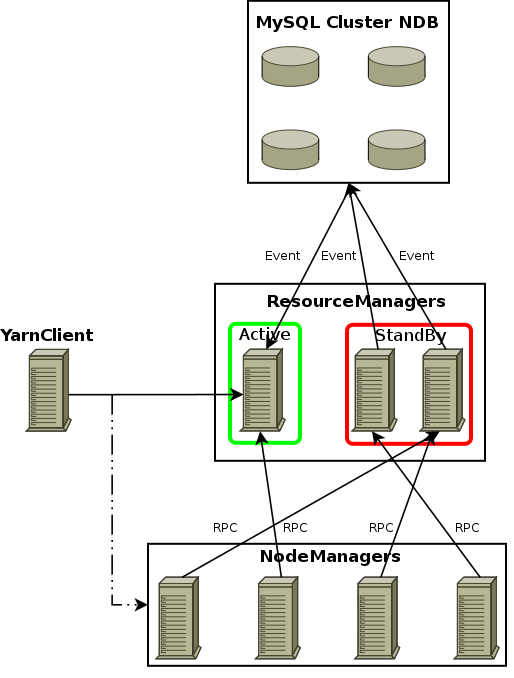
\includegraphics[scale=0.5]{resources/images/Background/hopsyarn_arch_overview.png}
\caption{Hops-YARN distributed RM architecture}
\label{fig:hopsyarn_dist_rm}
\end{figure}

\section{Taxonomy of schedulers}
\label{sec:taxonomy_of_schedulers}
Operating large-scale clusters is expensive both in terms of
investement to buy all the necessary hardware equipment but also in terms of
human resources that will maintain them. The variety in the jobs
running in a big organization poses a great challenge in the
utilization and efficiency of a cluster. There are long-running
production jobs that should ``never'' stop running, short-living
memory intensive batch jobs that analyze massive amount of data,
testing jobs running with the lowest priority and so forth. At the
same time schedulers should be able to scale to tens of thousands of
nodes per cluster and be highly available with minimum downtime. In order
to tackle these issues there has been a lot research regarding cluster
schedulers or datacenter operating systems as they are also
refered. In this section I will present three different architectures
identified in the current literature based on the taxonomy published
in the Omega paper \cite{41684}. An overview of these architectures is
depicted in Figure \ref{fig:sch_tax}.

\begin{figure}
\centering
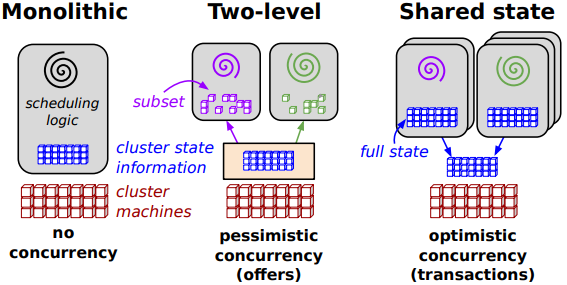
\includegraphics[scale=0.6]{resources/images/Background/schedulers_taxonomy.png}
\label{fig:sch_tax}
\caption{Cluster schedulers architecure \cite{41684}}
\end{figure}

\subsection{Monolithic}
\label{ssec:tax_monolithic}
The first category of schedulers explored is the \emph{monolithic}. In
this architecture there is a single, centralized entity that makes all
the scheduling decisions with no parallelism. A monolithic scheduler
still can facilitate different scheduling policies according to the type
of the workload by providing multiple code paths. Depending on the
type of the job, the execution flow can take different path --
policy. Although, it is tempting to support multiple
scheduling policies, ``it is surprisingly difficult to support a wide
range of policies in a sustainable manner using a single-algorithm
implementation'' \cite{41684}.

Another drawback of monolithic schedulers is the head-of-line
blocking. A small and easy to schedule job might get stack behind a
big and demanding job. This will delay the execution of the former, a
side effect that is not desirable in the enterprize world. Scalability
is another issue that has to be addressed. Since the scheduler runs on
a single instance it can be the bottleneck if the cluster size is big
enough. On the other hand, a monolithic scheduler has a full view of the
cluster and its available resources. For that reason it can make
optimal decisions on the job placement and achieving high utilization
(until it becomes the bottleneck).

A slight variation of a monolithic scheduler is the static
partitioning of the cluster. Each partition will run its own
monolithic scheduler with a separate policy according to the jobs
type. This approach though leads to fragmentation and to sub-optimal
cluster utilization.

A prominent example of a monolithic scheduler is Apache Hadoop YARN
and Hops-YARN. The key characteristic of Hops-YARN is that the state of the
scheduler is stored in the MySQL Cluster which opens the way for
various architectural experimentations resembling shared state schedulers (see
Section \ref{ssec:tax_shared_state}).

\subsection{Two-level}
\label{ssec:tax_two_level}
Two-level

\subsection{Shared state}
\label{ssec:tax_shared_state}
Shared state

\chapter{Methods}
\label{chap:methods}
The aim of this project is to minimize the time spent for Hops-YARN to commit
a transaction in the MySQL Cluster while at the same time parallelize the
process. This will increase the number of events processed by the
scheduler and the overall cluster utilization. In order to explore
the limits of the current system, different optimization techniques
were examined and evaluated as presented in Chapters
\ref{chap:implementation} and \ref{chap:evaluation}. For that reason a
\emph{Quantitative Research} method was followed. The impact of a new
feature in the system was measured in terms of commit time in the
database, the percentage of events handled by the ResourceManager or
the overall cluster utilization as suited.

The quantitative research method is supported by \emph{deductive}
approach and \emph{experimental} method. Before starting an iteration for
implementing a new feature, a thorough profiling of the
workflow of the system was performed, in order to identify the bottlenecks. Afterwards,
wherever it was possible, a prototype was created of the new
feature and benchmarked to validate any performance
gain. The micro-benchmark gave us an incentive on whether it was worth
investing on that feature or not. In case of a positive feedback,
a concrete version of the feature was implemented and finally the system's
performance was measured. After the completion of one feature, another iteration of the
procedure explained above took place to identify more bottlenecks in the system.

Regarding the data collection method, \emph{experiments} were
conducted throughout the project duration and with \emph{statistics}
data analysis calculation the results are presented in Chapter
\ref{chap:evaluation}. For the purpose of data collection a
cluster operated by SICS was used with seven physical machines and two MySQL
Clusters with four and two nodes respectively. In order for the
results to be \emph{reliable} each experiment run several times and
an average was computed where it was reasonable. Since the experiments took a
some time to finish and produced a lot of valuable data, custom
code to dump these data to files was employed and process them later. For the
\emph{validity} part of the experiments, a simulator was used that
simulated a configurable number of nodes in a Hadoop cluster and
measured in fixed intervals the variables that were interesting for
the system performance. After spawning the ResourceManager and the
ResourceTracker in multiple machines, it starts simulating the
NodeManagers that heartbeat the scheduler. Also, it parses existing
trace files and issues a synthetic workload to the scheduler. The simulator used is a
modified version of the simulator that ships together with the Hadoop
distribution. The difference is that the load of simulating the
NodeManagers and sending application launching requests is distributed across
multiple machines in the cluster. Since the workload is parsed from
trace files, it makes the experiments \emph{reproducible} by other
researchers. A note should be taken here. The performance of the system is affected
by the load of the physical machine, the network traffic and the
utilization of the database, so a small variation on the results
should be anticipated.


\chapter{Implementation}
\label{chap:implementation}
In this chapter I am going to present the work done throughout this
project. In Section \ref{sec:fk_constraints} I will present the
database schema that we were using in Hops-YARN and how this evolved
to a schema without any foreign key constraints yet being
consistent. Section \ref{sec:tx_aggregation} gives a detailed analysis
of the new transaction state manager of Hops and how that boosted our
performance. Section \ref{sec:gc_service} deals with the garbage
collector service written for Hops that deletes asynchronously old
data from the database. Finally, in Section \ref{sec:dto_caching} we
will explore the shortcomings of the MySQL Cluster connector for Java and
how we have managed to overcome them. As I have mentioned in Chapter
\ref{chap:methods}, each feature completion was followed by a system
profiling to guide us to the next bottleneck. The order of the
performance issues identified in the system is the same as the order
of the sections that follow.

Before diving into the implementation details I would like to give a
general overview of how Hops and Hops-YARN interact with the NDB
cluster in terms of Java packages. The interaction is illustrated in
Figure \ref{fig:impl_hops_ndb}. Hops distribution is statically linked
with the Data Access Layer (DAL) package \texttt{hops-metadata-dal}
which provides an API used by both Hops-HDFS and Hops-YARN to interact
with the persistent storage. Currently we have implemented a client
library for the MySQL Cluster NDB in the package
\texttt{hops-metadata-dal-impl-ndb} which also links to the DAL
package. Our choice in favour is the NDB cluster but users are free to
implement their own client library for any other storage solution as
long as the back-end has support for transactions, read/write locks and
at least read-committed isolation. Both Hops and the DAL API are
released under an Apache 2.0 license and the DAL implementation is
licensed under GPLv2.

\begin{figure}
\centering
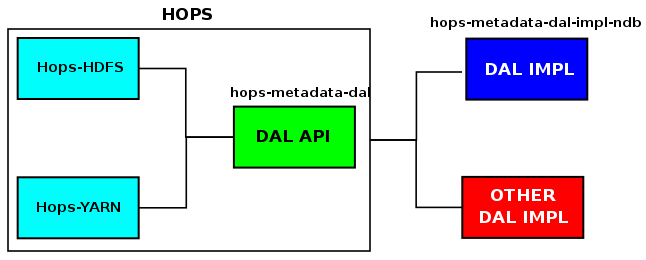
\includegraphics[scale=0.5]{resources/images/Implementation/hops_ndb_interaction.png}
\caption{Hops - MySQL Cluster interaction}
\label{fig:impl_hops_ndb}
\end{figure}


\section{Foreign key constraints}
\label{sec:fk_constraints}
In Hops for reasons that I have outlined in previous chapters we
persist all the metadata in our persistent storage solution. MySQL
Cluster is a relational distributed database, so data are stored into
tables with very specific properties. Since version 7.3.1, MySQL
Cluster supports foreign key constraints. Foreign keys is a powerful
feature of relational databases that guarantee some kind of
consistency between two tables. One important aspect of foreign keys
is that they map relationships of the ``real-world'' into
relationships in the database.

The database schema of Hops consists of 95 tables, 64 out of them are
used by Hops-YARN. The information they store span from incoming RPCs
to scheduler state and nodes' statuses. We make heavy use of foreign
key constraints, mainly the \texttt{ON DELETE} referential action, to
ensure integrity when a row from a parent table is deleted. Although
the database schema of Hops-YARN is too big to fit in
a single page, Figure \ref{fig:impl_fk_yarn_schema}, the number of
foreign key relationships -- they are illustrated with a solid line --
is clear. There our two reasons why we actually have relationships
between tables. The first one is because there is indeed semantically a
relationship between the tables. For example in Figure
\ref{fig:impl_fk_yarn_rmnode}, the table \texttt{yarn\_rmnode} is used by
the RM to store information regarding the available nodes in
the cluster. Table \texttt{yarn\_containerstatus} on the same figure
stores some status information for the containers that have been
launched. Obviously there is a relationship between the containers and
the nodes of a Hadoop cluster. A container cannot be launched in a
node that has not been registered with the RM yet. Similarly,
a container should not exists in the database if the node row has been
deleted. The second usage of foreign keys is to group together tables,
such as the tables in Figure \ref{fig:impl_fk_yarn_rpc}. These tables
persist the heartbeats sent by the AMs and NMs. For a reason that will
be explained in Section \ref{ssec:impl_fk_alloc_resp}, the information that a
single heartbeat carries had to be partitioned and stored in multiple
tables. Again, we do not want orphan entries and we avoid this by the
\texttt{ON DELETE} action.

Foreign keys in relational databases is a great feature. They do not
come without a cost though. For bulk and frequent operations they kill
performance. In our case that we want to scale to 10k nodes in a
cluster it means that we have to remove these constraints and replace
them with some logic in the program that will cascade the deletion to
children tables. It is very important that this logic will make
\textbf{primary key} operations for two reasons. The first reason, which
applies to all relational databases, is that primary keys are indexed,
so you avoid making full table scan. The indexes usually are
implemented with a \texttt{B-tree} data structure which allows
operations in logarithmic time. The second reason, which applies
specifically to NDB, is that primary keys are also partition keys. A
partition key defines how data will be distributed across Data Nodes
in the MySQL Cluster. Executing statements based on the primary key,
alleviates the round-trip time between the Data Nodes, since NDB will
know exactly in which machine the row you are looking for is
stored. In non primary key operations, NDB might have to lookup in all
Data Nodes to execute the statement.

Although the main reason we use foreign keys is to get the
automatic cascading in the deletion of a row, this has a side effect to
insertion operations also. A row in a child table cannot be inserted
in the database before its parent, otherwise the RDBMS will complain
about missing foreign key. To solve it we have to insert the parent
row, then \emph{flush} the buffer and then insert the child row which
imposes an order and cancels out any parallelism. In the rest of this section I will describe how I achieved
this for every parent table that had foreign keys to other children tables.

\begin{figure}
\centering
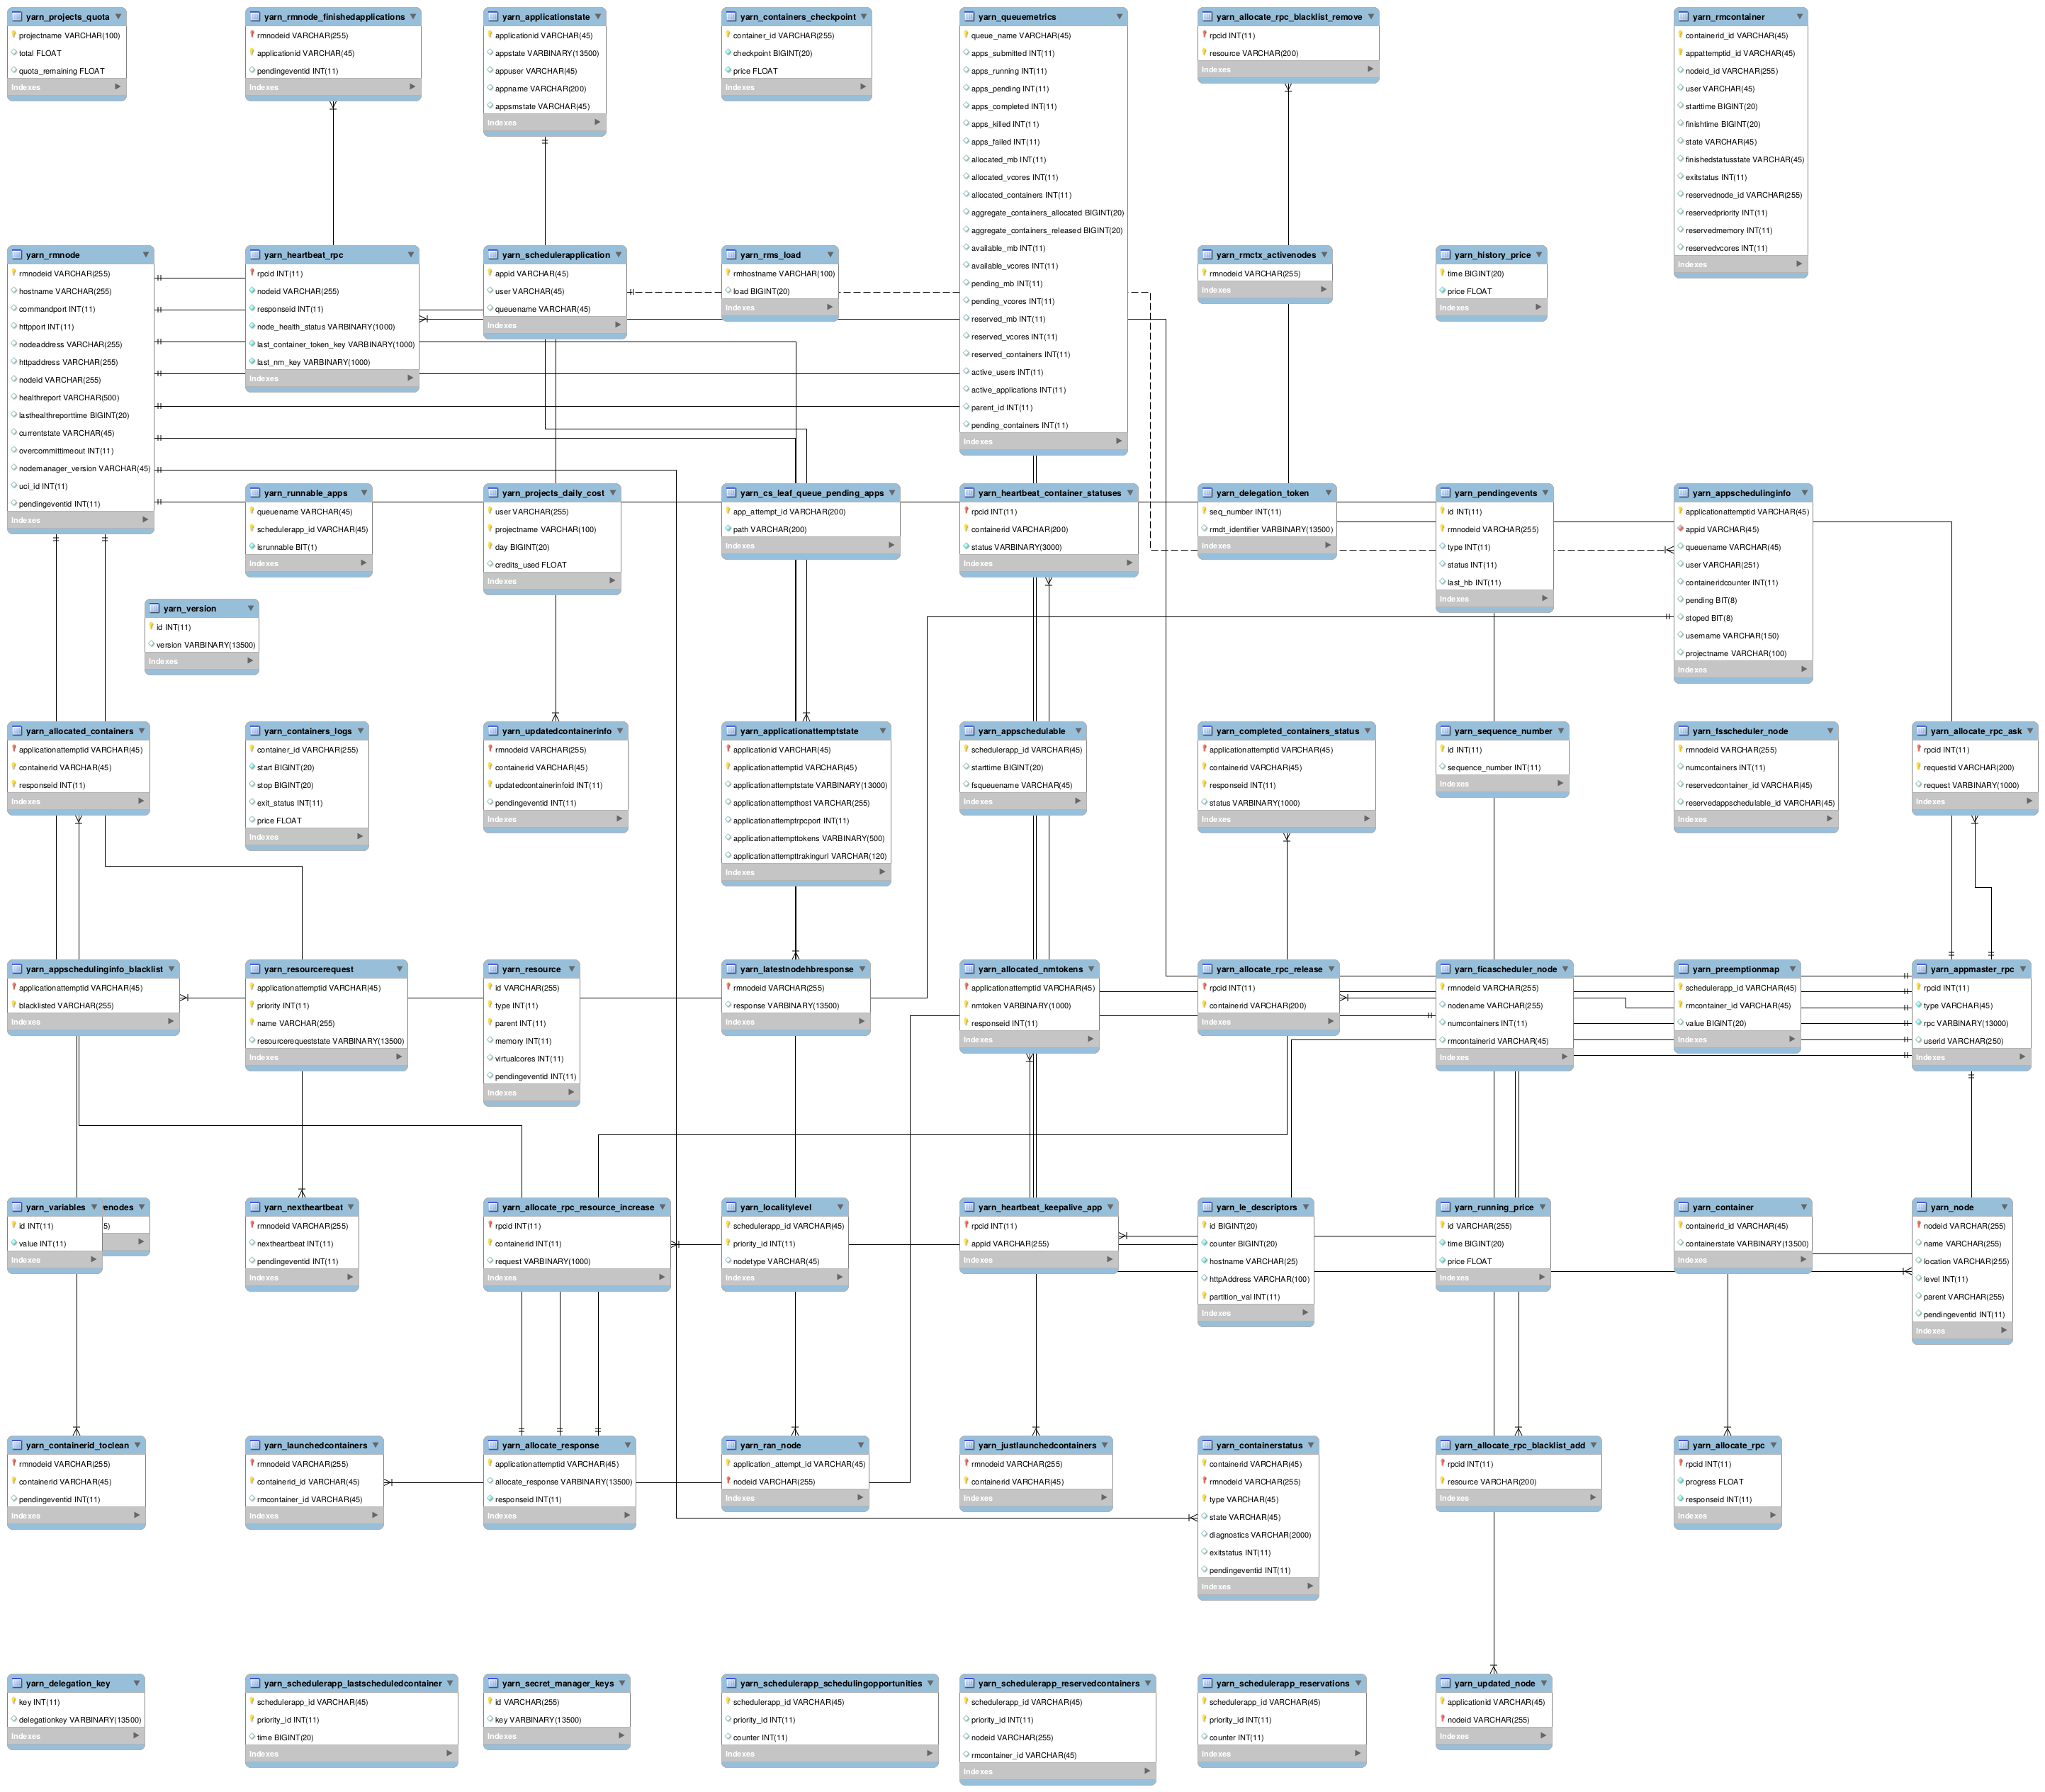
\includegraphics[scale=0.2,angle=90]{resources/images/Implementation/hops_yarn_ndb_schema_full.png}
\caption{Hops-YARN database schema}
\label{fig:impl_fk_yarn_schema}
\end{figure}

\begin{figure}
\centering
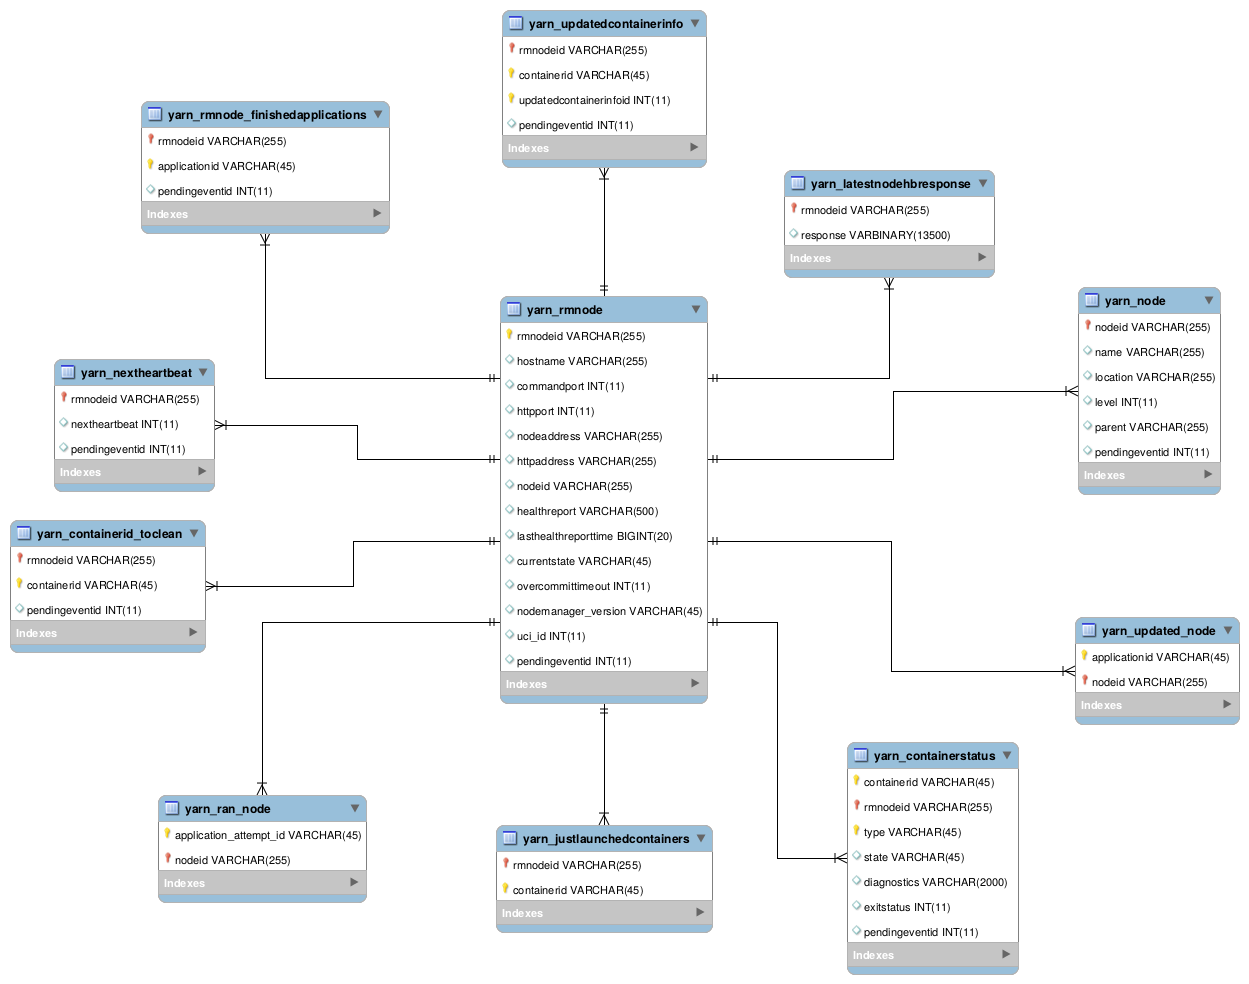
\includegraphics[scale=0.4]{resources/images/Implementation/hops_yarn_ndb_schema_rmnode.png}
\caption{A node in the cluster from the scheduler's perspective}
\label{fig:impl_fk_yarn_rmnode}
\end{figure}

\begin{figure}
\centering
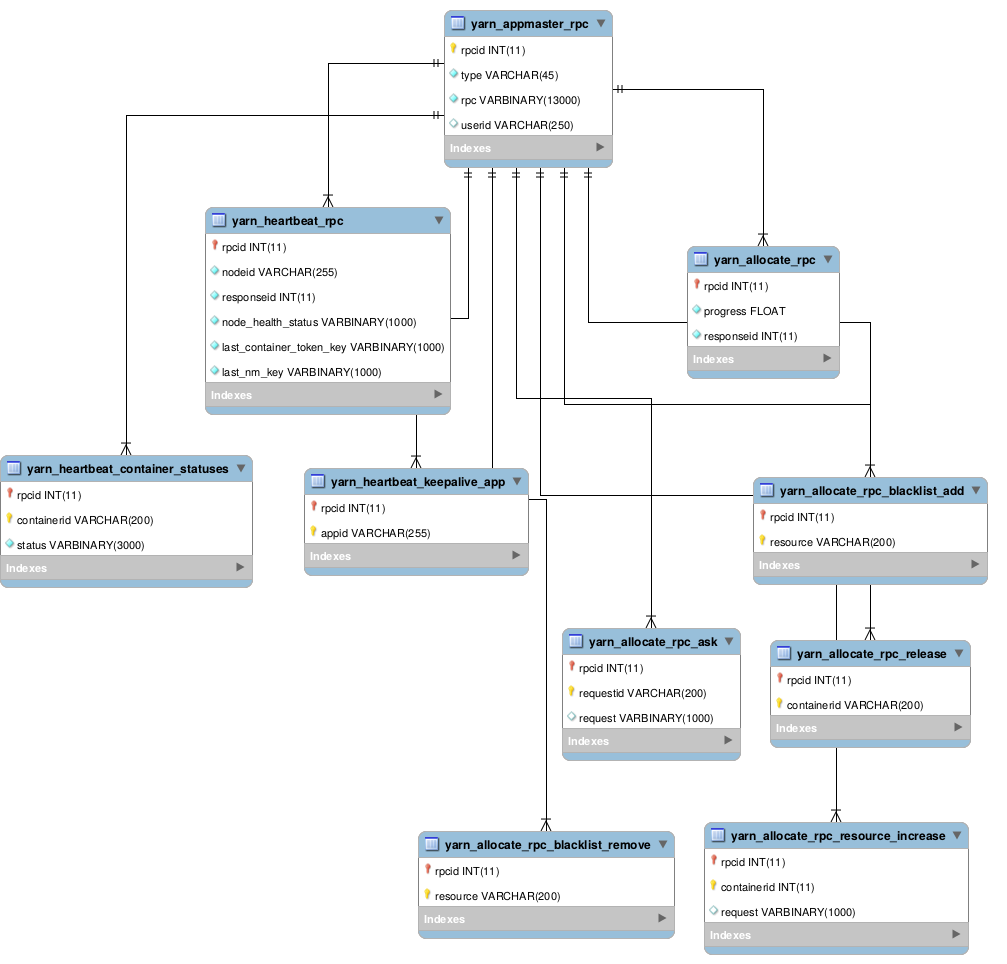
\includegraphics[scale=0.4]{resources/images/Implementation/hops_yarn_ndb_schema_rpc.png}
\caption{Database tables to store incoming RPCs}
\label{fig:impl_fk_yarn_rpc}
\end{figure}

\subsection{yarn\_rmnode}
\label{ssec:impl_fk_rmnode}
NodeManager is the process that runs on every physical node on a
Hadoop cluster. The scheduler keeps information for every NM
represented by the \texttt{RMNode} class. The information this
class holds is persisted in the \texttt{yarn\_rmnode} table, Figure
\ref{fig:impl_fk_yarn_rmnode}. This table is parent table to
numerous other tables such as \texttt{yarn\_node} which holds
information about the name of the node, its location etc. Another
table is
\texttt{yarn\_latestnodehbresponse} which holds the last response sent
by the RM to that NM. In total there are 10 tables having foreign key
constraints to \texttt{yarn\_rmnode}. Ideally we would like to replace
them with a logic that performs deletions with primary key
operations. The problem in that case is that the children tables are
diverse and have multi-column primary keys, so keeping in memory all
the primary keys would not be efficient. Especially when the deletion
operation of an RMNode would not happen very frequently, only in the case
of a dead node. Moreover, in later versions of YARN, RMNodes are never
removed from RM's state, just having their status changed.

With all these in mind we decided to remove the foreign key
constraints from the children without doing primary key
operations. In the client library we have implemented for NDB,
I wrote logic that whenever an RMNode row would be deleted, this
deletion would be cascaded to the rest of the tables. Children tables
have the \texttt{rmnodeid} either as part of their primary key or indexed, so we
avoid a full table scan. The implementation was very straightforward,
when the remove method in the client library is called for an RMNode,
I select all the rows from the corresponding tables filtered by the
\texttt{rmnodeid} and finally remove them. Considering that this
operation would occur rarely and in later versions never, that was a
fine solution trading performance with memory usage.

\subsection{yarn\_allocate\_response}
\label{ssec:impl_fk_alloc_resp}
Next in the list with tables that are referenced with foreign keys is
\texttt{yarn\_allocate\_response}. It holds the response sent by the
RM to an allocate request by an AM. This is the case where we had to
partition the data persisted. MySQL Cluster has a limit to the size of
a single row. That limit is 14000 bytes \cite{ndb_row_limit} and in
some cases the data that are to be persisted exceeds it. So the
allocation response is partitioned to
\texttt{yarn\_allocated\_containers} and
\texttt{yarn\_completed\_containers\_status}, both having foreign keys
to \texttt{yarn\_allocate\_response}. Since the deletion operation of
an allocate response would happen very often, primary key operation
was the only way to achieve high performance. Both tables have a
multi-column primary key with the \texttt{applicationattemptid}, the
\texttt{containerid} and the \texttt{responseid}. An allocate response
is removed from the database when $(1)$ a new response for that
application is created, $(2)$ the ApplicationMaster unregisters with
the RM. The first case will be examined in Section
\ref{sec:gc_service}. When an application unregisters I get all the
container IDs that the application was using from the RM in-memory
state and the response ID,
then I build the primary keys and issue primary key deletion
operations for those three tables in parallel.

\subsection{yarn\_ficascheduler\_node}
\label{ssec:impl_fk_fica_node}
The scheduler, and specifically Fifo and Capacity, holds information for the nodes in the cluster in its
own data structure identified by the class \texttt{FiCaSchedulerNode}. This
class is persisted in NDB in the table
\texttt{yarn\_ficascheduler\_node} which is parent for the table
\texttt{yarn\_launchedcontainers}. The later keeps a map of the
container IDs that are launched to a scheduler node. Its primary key
consists of the \texttt{nodeid} (FiCaNode) and the
\texttt{containerid}. The delete method on
\texttt{yarn\_ficascheduler\_node} Data Access Object is called when a
node is deleted from the scheduler's view. At that point the node
representation already holds the IDs of the containers that were
running on that node. Similarly, I construct the primary keys for the
child table for every \texttt{containerid} and issue the deletion operation for both
\texttt{yarn\_ficascheduler\_node} row and
\texttt{yarn\_launchedcontainers} rows.

\subsection{yarn\_applicationstate}
\label{ssec:impl_fk_appstate}
Hops-YARN persists in the database back-end the state of every
application scheduled. This state includes information such as the
name and the user of the application, the \emph{Application submission
  context}, diagnostics etc. Since applications and specifically AMs
can fail, YARN also tracks the attempts an application made to be scheduled.
If the AM fails, then YARN creates a new application attempt
for that application and spawns the new AM. The state of the
application is stored in \texttt{yarn\_applicationstate} table in the
database and every attempt for that application in
\texttt{yarn\_applicationattemptstate}. Application attempt
semantically has a relationship with the application and in the
relational world is expressed with a foreign key constraint
between \texttt{yarn\_applicationstate} (parent) and
\texttt{yarn\_applicationattemptstate} (child). When an application
is completed it is removed from the state of the scheduler and all
its attempts. Reconstructing the primary key for the attempts table
\texttt{<applicationid, applicationattemptid>} is trivial since the
application object holds the IDs of its attempts.

\subsection{yarn\_appschedulinginfo}
\label{ssec:impl_fk_appschedulinginfo}
An application from the scheduler's (Fifo, Capacity) point of view is
represented by the class \texttt{FiCaSchedulerApp}. This class
contains data structures that should be persisted such as resource
requests, the application attempt, any blacklisted resources etc. All
this information is stored in \texttt{yarn\_appschedulinginfo} table
which is parent to \texttt{yarn\_appschedulinginfo\_blacklist}
containing blacklisted resources for a specific application
attempt. In order to efficiently remove blacklisted resources when an
\texttt{yarn\_appschedulinginfo} row is removed, I have to construct
the primary key of \texttt{yarn\_appschedulinginfo\_blacklist} which
consists of the application attempt ID and the ID of the blacklisted
resource and then execute the delete operations.

\subsection{yarn\_schedulerapplication}
\label{ssec:impl_fk_schedulerapp}
\texttt{SchedulerApplication} class is the base class for
\texttt{FiCaSchedulerApp} that we have examined previously. This
naturally translates into a foreign key constraint between
\texttt{yarn\_appschedulinginfo} -- child, and \\
\texttt{yarn\_schedulerapplication} -- parent. In this case we have
three tables chained together with foreign keys. A deletion in table 
\texttt{yarn\_schedulerapplication}, will trigger a deletion in
\texttt{yarn\_appschedulinginfo} which in turn trigger a deletion in
\texttt{yarn\_appschedulinginfo\_blacklist}. This greatly deteriorates
the performance both for insert and delete operations. The foreign
keys dictate a very strict order on the insertion of rows in these
tables. If these statements are executed in parallel then there is no
guarantee about the order and an error might occur compromising the data. That
limitation forces us to excessively flush the buffer of the
transaction manager introducing network latency.

\subsection{yarn\_appmaster\_rpc}
\label{ssec:impl_fk_appmaster_rpc}
Finally, the last table that other tables had references to, was
\texttt{yarn\_appmaster\_rpc}. The database schema is illustrated in
Figure \ref{fig:impl_fk_yarn_rpc}. These tables are used to persist
incoming RPCs so in a crash scenario, the RM would recover and replay
them. At the time of replacing the foreign key relationships with
primary key operations we have decided to leave this set of tables as
it is. Later we saw that this setup was greatly affecting the
performance and the mechanism described in Section
\ref{sec:gc_service} came in place.

Having all, or most of, the foreign key constraints replaced by
primary key operations improved performance and made the database
schema more flexible. Performance was increased for two
reasons. Without any constraint we are able to remove the
\texttt{flush} operations from transactions. In some cases we do need
to maintain an order in our operations but that is limited. Removing
flushes allowed for increased \textbf{parallelism} in database operations while decreased the
network \textbf{latency} that we were paying for every flush
operation. In most of the cases, building the multi-column primary key
was an easy task but it was a great opportunity to get familiar with
YARN and NDB and a good warm-up for the changes to come.


\section{Transaction state aggregation}
\label{sec:tx_aggregation}
This section will present the new architecture of the Transaction
State manager of Hops-YARN. A \emph{Transaction State} in Hops-YARN is
an object that holds all the information that should be persisted in
the database back-end in a consistent way. Updates in the RM state are
generated either from heartbeats received from NMs and AMs or from
events that are streamed from the NDB event API (see Section
\ref{ssec:hops_yarn_load_balance}). Every modification in the
scheduler state should be reflected with updates in the corresponding
tables in NDB. Such modifications include:
\begin{itemize}
\item New applications that have been issued to the scheduler through
the YARN client. This include name of the application, user of
the application, the Application Submission Context, state of the
application etc.

\item New application attempts including reference to AM,
diagnostics, list of nodes that the containers of this application run
etc.

\item Newly created containers that applications will use

\item Containers that have finished their job and should be removed
from scheduler's state

\item Containers that have updated their state for some reason etc.

\item Newly added nodes in the cluster
\end{itemize}

For the full list of the modifications tracked and persisted in NDB,
consult \texttt{TransactionStateImpl.java}
\footnote{\url{https://goo.gl/Ukq4Tp}} file.

It is important that the state persisted in the database reflects the
state of the ResourceManager in memory. In case of a recovery, the
state recovered should be the last known state and be consistent. An
example of inconsistency would be a container to be listed as running
even though the application that was using it has finished. In order to
avoid such situations and achieve the consistency level we desire
there is the notion of Transaction State (TS). A TS is committed in an
``atomic'' fashion. This is facilitated by the transactional nature of
MySQL Cluster, so a commit of one TS is one ``big'' SQL
transaction. Using transactions we achieve isolation and atomicity of
our Hops TS. With the all-or-nothing architecture of transactions, if
the RM crashes in the middle of a commit, then the whole TS will be
aborted. Similarly, in case of an error during the commit phase it will
roll-back the whole transaction leaving the database in a clean state.
More information regarding how a TS is created is presented in Section
\ref{ssec:impl_batch_system}. Having our safety property covered, one
more reason to use Transaction States is for efficiency. Committing a
single Transaction State with a lot of modifications is more efficient
than committing small modifications several times.

The Transaction State is implemented generally with concurrent hash maps and
accessors in the style of \texttt{add*ToAdd} for entries that we
want to persist in the database and \texttt{add*ToRemove} for entries
that we want to delete from the database. Even inside a TS we should
be very careful on how we access the fields. A TS holds modifications
from several RPC requests that may modify the same element. For
example one RPC might create a new container and the next one to
destroy it. YARN internals are event-based. So there is no guarantee
about the order that events will be processed. The second RPC might
follow a different code path and finish earlier than the first one. In
that case what will be persisted in the database would be the creation
of a new container, something completely wrong. That is the reason
we hold two separate data structures for the same table, one for
insert operations and another for delete operations. First the insert
data structure is processed that persists entries in the database and
then the delete data structure.

Section \ref{ssec:impl_batch_system} will give some insights on
the existing batching system, while in Section
\ref{ssec:impl_aggr_mechanism} the new queuing
mechanism will be presented that improved the commit time.

\subsection{Batching system}
\label{ssec:impl_batch_system}
So far we have discussed why we need the Transaction State in
Hops-YARN and how it is implemented. We still miss the part of how
Hops-YARN handles heartbeats or events from NDB and how the scheduler
updates the fields in it. A TS object is managed by the
\emph{TransactionStateManager} a custom service that runs on Hops-YARN.
It is responsible for creating new TS, provide the
current TS to methods that have requested it and keep track of how many
RPCs have requested the TS.

Heartbeats from AMs and NMs from the side of RM are perceived as
RPCs. Upon an RPC, the method invoked will ask for the TransactionStateManager
to provide the current TS. The TS will be piggybacked to every event
triggered by RM components and ``travel'' all the way until that
request has been fully handled. Each modification made by the components
to the state of the RM will also be added to the insert and delete
data structures explained above. TransactionStateManager service
provides isolation by batching several RPC requests together, let the
requests be handled and then batch the next RPCs in a different
TS. The activity diagram of the batching system is depicted in Figure
\ref{fig:impl_rpc_batch_system}.

\begin{figure}
\centering
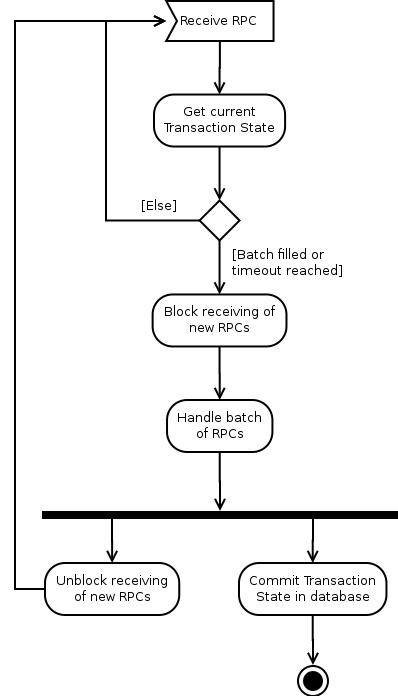
\includegraphics[scale=0.4]{resources/images/Implementation/rpc_batch_system_activity.png}
\caption{Activity diagram of RPC batching system}
\label{fig:impl_rpc_batch_system}
\end{figure}

At the beginning the TransactionStateManager service creates a
Transaction State object. Heartbeats start coming from the
ApplicationMasters and the NodeManagers in the form of RPCs. The
methods that are invoked, get the current TS from the
TransactionStateManager and piggyback them to the events
triggered, while various RM components handle those events in separate
threads.
The TransactionStateManager service keeps receiving RPCs
until a certain threshold of received RPCs -- default is 60, or until
a timeout has been reached -- default is 60 ms. At the point where
either of two is satisfied, it blocks responding to further
\texttt{getCurrentTransactionState} requests until all the RPCs in the
previous batch have been handled properly and put in the queue to be
committed in the database back-end. When this is done, it
creates a new Transaction State object and unblocks the receiving of
new RPCs. At the same time but in a \textbf{different thread}, the previous
Transaction State is committed to the database as described in Section
\ref{ssec:impl_aggr_mechanism}.

In Hops-YARN we have distributed the \emph{ResourceTrackingService} to
multiple machines in the cluster. They receive heartbeats from the
NodeManagers and persist them in NDB. MySQL Cluster has an event API
that can stream events to subscribers. In RM there is a custom C++
library that receives the events emitted from NDB, creates a Java
representation of them and put them in FIFO queue. In the background
there is a Hops service that polls from the queue and triggers the
appropriate events. The Transaction State is also included in these
events as the cascading modifications should be persisted in the
database. The same Transaction State manager service is used as
described in the previous paragraph, so from the manager's perspective
there is no difference between RPC events and NDB events.

\subsection{Aggregation mechanism}
\label{ssec:impl_aggr_mechanism}
Heartbeats arrive in the RM and invoke specific methods. The methods
invoked create specific events which include the TS and are sent to an
event dispatcher thread. The event dispatcher will forward the events
to the appropriate RM components that will trigger some actions and
probably create more events. All along the ``journey'' of these
events, TS track all the necessary modifications that should be
persisted in the database back-end. After all events in a batch have
been properly handled they should be committed in NDB.

Persisting in a non-volatile storage solution is expensive due to
exclusive locks, OS buffers, I/O interrupts etc. On top of that,
persisting data in a remote database, introduces a
few milliseconds of network latency as well. For that reason,
when a TS is ready to be committed, it forks
a new thread which will handle the actual database operations to
persist its state. Having the commit mechanism parallelized, multiple
TS can be persisted concurrently. At that point, we have just
invalidated our consistency model. Sooner or later we will
reach the case where two TS would be committed in the wrong order
corrupting the state of the database. The mechanism explained in
Section \ref{sssec:impl_aggr_old} controls the commit phase of each TS
guarantying that two conflicting TS will be committed in the correct
order. Section \ref{sssec:impl_aggr_new} will outline the
shortcomings of the existing mechanism and describe the new mechanism
built that extends the previous.

\subsubsection{One TS per commit}
\label{sssec:impl_aggr_old}
The mechanism that controls the commit phase of TS should allow as
much as possible parallelism without violating our constraints. The
constraints are:
\begin{itemize}
\item If the RPCs that are batched in Transaction State $TS_0$ have
  been fully handled before the RPCs batched in $TS_1$ and they both
  modify the same \textbf{YARN Application}, then the commit phase of $TS_0$
  should have been successfully completed \textbf{before} the commit
  phase of $TS_1$ begins

\item If the RPCs that are batched in Transaction State $TS_0$ have
  been fully handled before the RPCs batched in $TS_1$ and they both
  modify the same \textbf{NodeManager}, then the commit phase of $TS_0$
  should have been successfully completed \textbf{before} the commit
  phase of $TS_1$ begins

\item If Transaction States $TS_0$ and $TS_1$ modify different YARN
  Application \textbf{and} different NodeManager, they should be committed in parallel
\end{itemize}

Every TS keeps a list with the IDs of the applications it modifies and
a list with the IDs of the nodes it modifies. In the commit mechanism,
there is a FIFO queue for each and every application ID and node
ID. Before committing a TS, the mechanism puts it in the corresponding
queues both for the applications and the nodes it modifies. Then it
gets the IDs of the applications and nodes it modified. In order for
the TS to be committed, it should be in the \textbf{head} of the
queues for the corresponding application IDs \textbf{and} node IDs. If
it is not in the head of one application or node queue, it means that
a previous TS modified the same application or node and should be
committed before. The un-committed TS is put in a queue to be
examined later.

The following example will make clearer how the commit mechanism works.
To make it easier, let us assume that the only lock is on
application IDs and we have only three applications running. The FIFO
queues for the applications are depicted in Figure
\ref{fig:impl_tx_aggr_queue}. The initial state of the system is in
Figure \ref{fig:impl_tx_aggr_sub0} where no TS has been handled yet
and the queues are empty. Technically, the queues for the application
IDs and node IDs are created lazily when the TS has been fully handled
and is ready to be committed. RPCs for \texttt{TS\_0} have been
handled and is ready to be committed in the database. It modifies
entries for applications with ID \texttt{app\_0} and \texttt{app\_2},
so it is placed in the respective queues, Figure
\ref{fig:impl_tx_aggr_sub1}. \texttt{TS\_0} is the head
of the queues for the applications it modifies so it can start the
commit phase. Since a commit phase may fail and roll-back, it will be
removed from the queues when the transaction has been successfully
completed.

While \texttt{TS\_0} tries to persist its modifications to the
database, two more Transaction States have finished and are put in the
queue to be committed, Figure
\ref{fig:impl_tx_aggr_sub2}. \texttt{TS\_1} modifies applications
\texttt{app\_0} and \texttt{app\_1} while \texttt{TS\_2} modifies
applications \texttt{app\_1} and \texttt{app\_2}. The commit mechanism
checks whether \texttt{TS\_1} can be committed. Remember that
\texttt{TS\_0} is still committing to the database. The mechanism
fetches the applications that \texttt{TS\_1} modifies and checks if it
is the head in each queue. For \texttt{app\_1} it is in the head of
the queue but not for \texttt{app\_0}, \texttt{TS\_0} should finish
first. So it will be examined after \texttt{TS\_0} is done. The same
applies for \texttt{TS\_2}.

\texttt{TS\_0} is now complete and removed from the queues of the
applications it modified, Figure
\ref{fig:impl_tx_aggr_sub3}. \texttt{TS\_1} is now the head for
\texttt{app\_0} and \texttt{app\_1} so it starts the commit
phase. This is not the case though for \texttt{TS\_2} which still has
to wait for \texttt{TS\_1} to finish. \texttt{TS\_1} successfully
completes its transaction, removed from the queues and now
\texttt{TS\_2} is in the head position, Figure
\ref{fig:impl_tx_aggr_sub4} so it can start committing to the database.

\begin{figure}
  \centering
  \begin{subfigure}[t]{0.3\textwidth}
    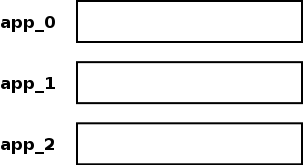
\includegraphics[scale=0.4]{resources/images/Implementation/commit_system_0.png}
    \caption{}
    \label{fig:impl_tx_aggr_sub0}
  \end{subfigure}
  \hfill
  \begin{subfigure}[t]{0.3\textwidth}
    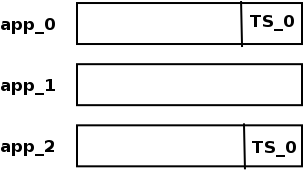
\includegraphics[scale=0.4]{resources/images/Implementation/commit_system_1.png}
    \caption{}
    \label{fig:impl_tx_aggr_sub1}
  \end{subfigure}
  \hfill
  \begin{subfigure}[t]{0.3\textwidth}
    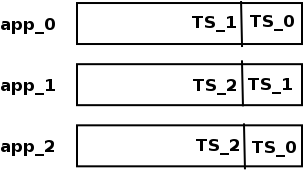
\includegraphics[scale=0.4]{resources/images/Implementation/commit_system_2.png}
    \caption{}
    \label{fig:impl_tx_aggr_sub2}
  \end{subfigure}
  \\[2em]
  \begin{subfigure}[t]{0.3\textwidth}
    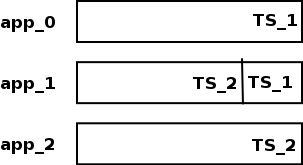
\includegraphics[scale=0.4]{resources/images/Implementation/commit_system_3.png}
    \caption{}
    \label{fig:impl_tx_aggr_sub3}
  \end{subfigure}
  \qquad
  \begin{subfigure}[t]{0.3\textwidth}
    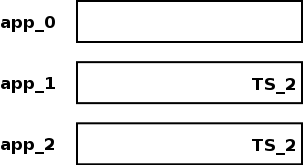
\includegraphics[scale=0.4]{resources/images/Implementation/commit_system_4.png}
    \caption{}
    \label{fig:impl_tx_aggr_sub4}
  \end{subfigure}

  \caption{Example of TS for the queue to be committed}
  \label{fig:impl_tx_aggr_queue}
\end{figure}

\subsubsection{Multiple TS per commit}
\label{sssec:impl_aggr_new}
The existing mechanism described in the section above provided the
consistency model we required and parallelism for
non-conflicting TSs. The major issue that had to be addressed was that
for conflicting TSs $(1)$ they had to wait in the queue for another TS
to finish, in the example above \texttt{TS\_1} and \texttt{TS\_2} and
$(2)$ for every transaction committed we paid the network latency
penalty and the time probably to acquire locks etc. In order to solve
the first problem we examined different solutions. Initially,
a more fine-grained locking system was tried. Instead of locking on application and
node IDs, try to lock on containers. Although this solution would
increase parallelism, it was very risky that we would end-up with a
corrupted state. Next solution was to remove the system with the
queues and replace it with exclusive reentrant locks. The expected
result was to increase performance but at the end it was the same.

The solution proposed in this section and implemented reduces both the
wait time in the queue for a TS to be committed and the RTT for each
transaction performed. The mechanism extends the method described in
Section \ref{sssec:impl_aggr_old} by aggregating multiple TSs into a
single one while it guarantees consistency. The queue system still
gives us the proper order in which the TSs should be persisted. At the
beginning a TS
is examined if it should be persisted in the database. If it is not
possible to be persisted due to conflicting TSs then it is put in the
\emph{toBeAggregated} set. If it is permitted to commit, then it does so
and constructs an extended TS called
\emph{AggregatedTransactionState}.

The \emph{AggregatedTransactionState} contains TSs from the
\emph{toBeAggregated} set that are eligible for commit according to the
following aggregation rules:
\begin{enumerate}
  \item A TS was not the head in its respective queues at the time it
    was examined for commit, but until now the conflicting TS(s) have
    been committed and removed. So now it is in the head of the
    queues.

  \item A TS is still not in the head of the queues, but all the
    conflicting TSs that should be committed before, have already been
    aggregated in the \emph{AggregatedTransactionState}.
\end{enumerate}

The first rule is trivial and we have examined it in the previous
section. For the second rule, the mechanism gets the modified
application and node IDs from a Transaction State \texttt{TS\_a}.
Then it retrieves all the conflicting TSs from the appropriate queues
that are blocking \texttt{TS\_a} from being committed. If all of the
conflicting TSs have already been aggregated -- put in the
\emph{AggregatedTransactionState}, then the mechanism aggregates
\texttt{TS\_a} as well and it proceeds by examining the next TS in the
\emph{toBeAggregated} set. At the end of this process we will end-up
with a ``big'' Transaction State, the
\emph{AggregatedTransactionState} that will be committed in the
database. The \emph{AggregatedTransactionState} class actually extends
the \emph{TransactionState} class and for every TS that is aggregated
it updates the data structures with the modifications of that TS. The
\emph{toBeAggregated} data structure is a FIFO queue so the TSs that
are examined for aggregation are kept in the correct order. At the
end of the aggregation process, the data structures of the
AggregatedTransactionState hold the correct, most recent, modifications to be persisted.

Consider the state of the queues as in Figure
\ref{fig:impl_tx_aggr_sub2}. Both \texttt{TS\_1} and \texttt{TS\_2}
cannot be committed because they are blocked by \texttt{TS\_0} so they
are added to the \emph{toBeAggregated} queue. At some
point \texttt{TS\_0} is committed in the database, removed from the
queues as in Figure \ref{fig:impl_tx_aggr_sub3}, creates the
\emph{AggregatedTransactionState} (ATS)
and starts the aggregation process. \texttt{TS\_1} is the first
candidate for aggregation. At that point \texttt{TS\_1} is at the head
of its respective queues and following the aggregation rule $1$ it is
aggregated. All the data structures of \texttt{TS\_1} are copied to
the data structures of the ATS. Next in the \emph{toBeAggregated} set
is \texttt{TS\_2}. \texttt{TS\_2} is not the head in the queue for
application \texttt{app\_1} but the conflicting TS, \texttt{TS\_1}, has
already been aggregated. So according to aggregation rule $2$,
\texttt{TS\_2} is also aggregated, probably updating the values that
\texttt{TS\_1} has put in TSA. The \emph{toBeAggregated} set is now
empty and the ``big'' AggregatedTransactionState is committed to the
database. Compared to the existing commit mechanism, where we have
done three commits in the database, we have now reduced it to two.

\begin{figure}
\centering
\begin{subfigure}[t]{0.3\textwidth}
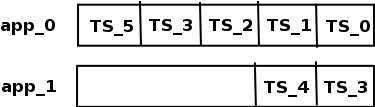
\includegraphics[scale=0.4]{resources/images/Implementation/commit_system_aggr_example.png}
\caption{}
\label{fig:impl_tx_aggr_ex0}
\end{subfigure}

\begin{subfigure}[t]{0.3\textwidth}
  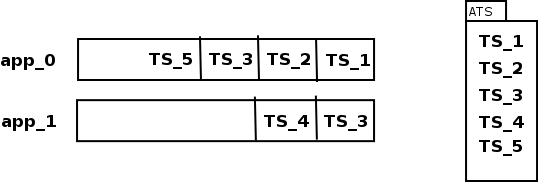
\includegraphics[scale=0.4]{resources/images/Implementation/commit_system_aggr_example_1.png}
  \caption{}
  \label{fig:impl_tx_aggr_ex1}
\end{subfigure}
\caption{Aggregate commit mechanism example}
\label{fig:impl_tx_aggr_example}
\end{figure}

Another case that demonstrates the improvement we have achieved is
described in the following example. Consider the locking queues as
depicted in Figure \ref{fig:impl_tx_aggr_ex0} for two applications. All the Transaction
States are blocked behind \texttt{TS\_0} which is at the commit
phase. At that time the \emph{toBeAggregated} set contains
\texttt{TS\_1}-\texttt{TS\_5}. \texttt{TS\_0} finishes its commit phase, removes
itself from the locking queues and begins the aggregation phase. First
it examines \texttt{TS\_1}. It is in the head of the queue for
application \texttt{app\_0} and according to aggregation rule $1$ it
should be aggregated. Next in the \emph{toBeAggregated} set is
\texttt{TS\_2}. The conflicting state is \texttt{TS\_1}, which is
already aggregated, so according to aggregation rule $2$ it is
aggregated too. \texttt{TS\_3} is in the head of the queue for
\texttt{app\_1} and all the conflicting TSs for \texttt{app\_0} have
been aggregated so it is also put in the
\emph{AggregatedTransactionState}. Similarly, \texttt{TS\_4} and
\texttt{TS\_5} are also aggregated. Now the
\emph{AggregatedTransactionState} contains the modifications of
\texttt{TS\_1}, \texttt{TS\_2}, \texttt{TS\_3}, \texttt{TS\_4},
\texttt{TS\_5}, Figure \ref{fig:impl_tx_aggr_ex1} and begins the commit phase. With the previous commit
mechanism, every TS would have performed the commit phase individually introducing
considerable delay due to the RTT to the database, whereas with the
new commit mechanism we only require two commits in the database.

Aggregating several TSs into a single one introduced some erroneous
behaviour. NDB is very performant with transactions of small size but
the aggregation mechanism was overloading the transaction and NDB was
throwing errors. In order to mitigate this issue a TCP-like aggregation control
was put in place. In the beginning, the mechanism starts to aggregate
a small number of TSs. When the commit phase for that
\emph{AggregatedTransactionState} is successfully completed, the limit
is increased by some delta. It continues to increase until an error
message is received from the database. The transaction is rolled-back,
the limit for the number of aggregations is set to minimum and the
mechanism tries again to aggregate. Users can implement their own
policy as it fits their needs without having to change the commit
mechanism code.

Overall, the new commit mechanism addresses both the waiting time in
the queue and the communication latency. TSs do not have to wait in
the queue for all the conflicting TSs to be committed. Once one
conflicting TS is committed then the mechanism aggregates as many as
possible TSs. Moreover, since multiple TSs are squashed into a single
one, there is only one commit phase reducing the network latency.


\section{Garbage Collector service}
\label{sec:gc_service}
Analyze the GC service

\section{DTO Caching mechanism}
\label{sec:dto_caching}
In Hops in order to communicate with the MySQL Cluster NDB we make use
of ClusterJ \cite{clusterj}, a high level API for performing
operations on NDB. In a sense it is similar to other ORM frameworks
such as Hibernate \cite{hibernate} and EclipseLink \cite{eclipselink}
which provide an object-relational mapping but more lightweight and is
designed to provide high performance methods for storing and accessing
data on a MySQL Cluster from a Java application. Every operation on
Hops and Hops-YARN, except for the events received from the NDB Event
API, goes through ClusterJ which in turn uses the C++ NDB API. The
mapping between a table-oriented view and a Java object is done
through specially decorated interfaces. The interface must also provide signatures
for the getters and setters methods.

For example in Listing \ref{lst:clusterj_intf} is the interface for
accessing database entries for the Garbage Collector service regarding
old RPCs. The interface is annotated with the table name and contains
signatures for accessing each column of the table. The methods are
also decorated with the primary key annotation and the column
name. For every table in the database there exists such an interface
and all the operations from the Hops-YARN are done on objects defined
by the annotated interfaces. \emph{Data Transfer Object}s (DTOs) are
created from a \emph{session} object which represent a connection to
the MySQL Cluster by calling the \texttt{newInstance} method. In a
typical setup an application would have multiple sessions to the
cluster. 

\lstinputlisting[float,language=Java,frame=single,caption={ClusterJ
annotated interface},label=lst:clusterj_intf]{resources/listings/clusterj_intf.java}

Upon completion of the task discussed in the previous section, we
profiled again the commit phase of a Transaction State to discover
spots where we could possibly improve. Surprisingly we discovered that
we suffered from the overhead of creating DTOs with ClusterJ. Looking
at the results of a micro-benchmark that created and persisted a
number of DTOs was astonishing. In Figure \ref{fig:impl_dto_no_cache},
the blue line represents the time that ClusterJ needed to create the
DTO instances when calling \texttt{session.newInstance}. The yellow
line is the actual time we spent just to persist them in NDB, while
the red one is the sum of those two. Constantly we are spending more
time creating the object instances than actually persist
them. Especially, when the number of instances grows beyond 6000 the
difference is massive. Creating more than 6000 DTOs is not an extreme
scenario when we are aiming to scale Hops-YARN over 10000
NodeManagers.

\begin{figure}
\centering
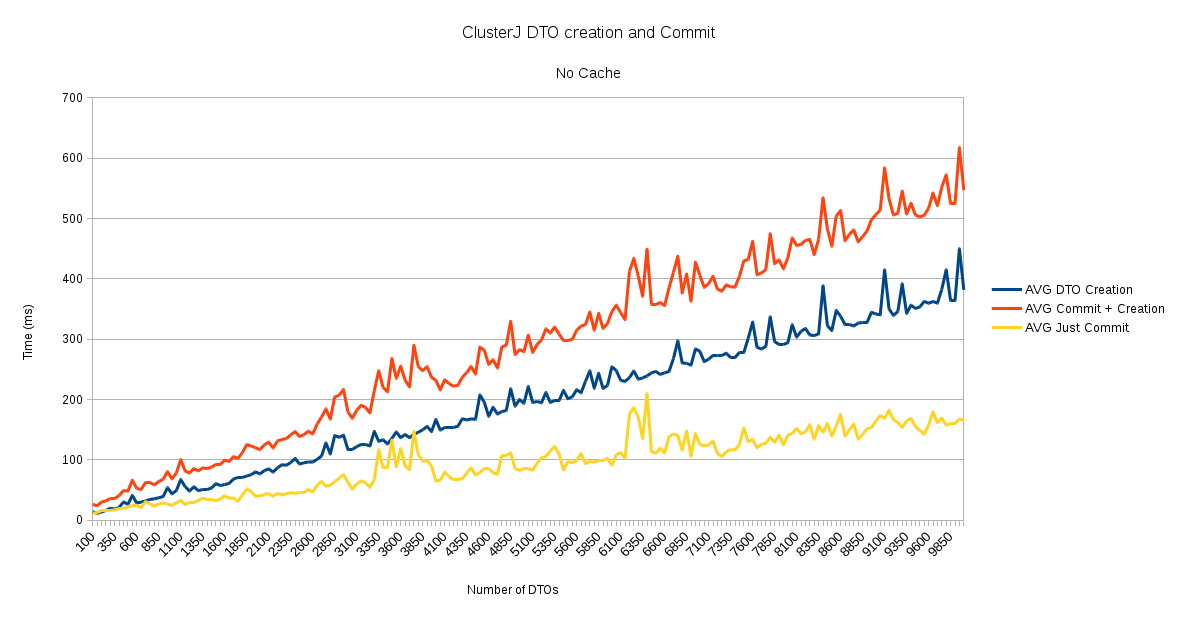
\includegraphics[scale=0.55]{resources/images/Implementation/dto_create_commit_no_cache.png}
\caption{Create and commit time for simple DTOs}
\label{fig:impl_dto_no_cache}
\end{figure}

In ClusterJ, DTOs are created from \emph{session} instances. Creation
of a new instance involves the creation of several objects such as the
handlers for the type of values the DTO will persist in NDB. Upon creation
of all the necessary handlers to check the types, it invokes the
\texttt{newInstance} reflective method of Java. Java reflection API is
a powerful tool but comes with some pitfalls including
performance \cite{java_reflection}. Reflection API loads types dynamically therefore JVM
optimizations cannot be applied making it not a good candidate for
high-performance applications. Changing the implementation of ClusterJ
is a very difficult task and was not considered as an
option. Moreover, we do not want to maintain one more project.

In Hops, ClusterJ sessions are wrapped around \emph{HopsSession}s. The
solution we designed was a DTO cache for the sessions we were
using. A session would have each own cache space that would be filled
up with instances created by the ``slow'' ClusterJ instantiation
process. When we actually needed to use a DTO, we would fetch it from
the cache which is faster since the objects would have already been
created. When the cache has been used a worker thread would fill it up
again with new instances. The cache generator service should be used
cautiously. We should not max-out CPUs just for creating cached DTOs, so the
cache would be enabled only for a fraction of sessions and only for
heavy-duty DTOs. The reason why we decided to have both cache-enabled
and cache disabled sessions, was that we did not want to pay the
cache-miss penalty for the type of DTOs that we already know we do not
cache. An overall architecture of Hops-YARN database session provider
is illustrated in Figure \ref{fig:impl_dto_session_arch}. A
transaction requests a cache-disabled session from the cache-disabled
session pool $(1)$. If there is a session available -- not used by
other transactions -- then the session provider return a session from
the pool, otherwise it creates a new one. When the transaction has
been committed to the database, the session is returned back to the pool
of cache-disabled sessions $(3)$.

The workflow for a cache-enabled session regarding the provider is
slightly different. There are two different cache-enabled session
pools. The first one, \emph{Preparing pool} contains sessions with
their cached used and probably empty. The second pool is the
\emph{Ready pool} with sessions whose cache is full and ready for
usage. When a transaction requests a cache-enabled session, the session
provider first looks on the \emph{Ready pool} $(1)$. If there is an
available session it returns it to the requester $(2)$, otherwise it
looks into the \emph{Preparing pool}. Finally, if there is no session
there either, it creates a new session to NDB. When the transaction
has performed its operations, it returns the session to the
\emph{Preparing pool}. The cache generator service picks sessions from
the \emph{Preparing pool} $(1)$, fills up their cache with the appropriate
DTO instances and places them back to the \emph{Ready pool} $(2)$.

\begin{figure}
\centering
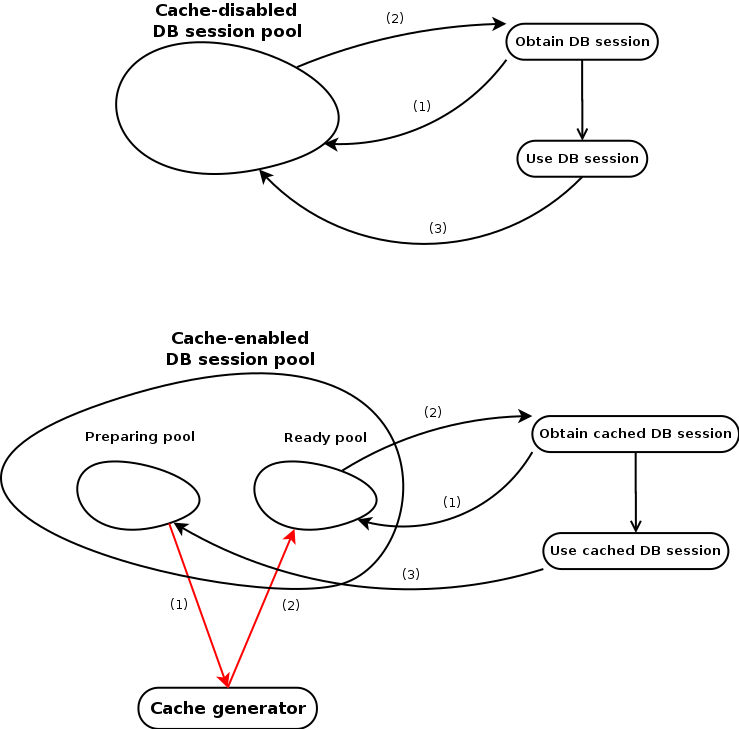
\includegraphics[scale=0.4]{resources/images/Implementation/db_session_pools.png}
\caption{Hops-YARN DB session pool}
\label{fig:impl_dto_session_arch}
\end{figure}

The cache itself, \texttt{DTOCacheImpl} is implemented as a \texttt{ConcurrentHashMap} whose
key is the type of DTO cached and its value is a \texttt{CacheEntry}
object. The \texttt{CacheEntry} is supported by an
\texttt{ArrayBlockingQueue} providing methods for putting and getting
cached objects and increase the cache size. We will see later how
the size of the cache is increased. For every \texttt{HopsSession}
that has its cache enabled, there is an instance of
\texttt{DTOCacheImpl} which provides methods for (de)registering a DTO
type to the cache and methods that delegate putting and getting to the
appropriate \texttt{CacheEntry}. To avoid the cache-miss penalty there
two ways to ``instantiate'' DTO objects. The first one is the
\texttt{newInstance} which makes a call to ClusterJ to create the
object. We use this for non-cached DTO types. The other variation is
the \texttt{newCachedInstance} which makes a call to the cache
instead. Apparently in this version, the DTO has been instantiated
ahead of time and it is fetched from the cache. The semantics of the
cache is returning the cached object if
it exists in the cache and \texttt{null} if the cache is empty. In
case of an empty cache, we fall back to the ClusterJ instantiation
method. Every \texttt{CacheEntry} keeps track of how many cache-misses
have been occurred. If there are too many, it means that this DTO type
is very demanding and the cache size is increased every time the
cache-misses exceed a certain threshold. So, at the same cache-enabled
session two DTO types might have different cache size depending on
their ``popularity''.

When a cached-enabled session has been used, it is put back in the
\emph{Preparing pool}. The \texttt{DTOCacheGenerator} is a service
that picks sessions from that pool and fills their cache. It removes a
number of session from the \emph{Preparing pool} and it spawns threads
that will populate every \texttt{CacheEntry} that is not
full. The instantiation of the cached DTO objects is done with the
\texttt{newInstance} method of ClusterJ. \texttt{CacheEntry} returns
\texttt{true} for every put, until
the back-end \texttt{ArrayBlockingQueue} is full and returns
\texttt{false}. When all the \texttt{CacheEntry}s of a session are
full, it (session) is placed to the \emph{Ready pool} and another
transaction will use it. One note should be made here. ClusterJ
allocates memory for DTO objects out of the heap, with the use of
Java \emph{direct} ByteBuffer. ByteBuffers do not account in Java's
garbage collection mechanism, reducing the GC pause time. Also, they are ideal
for heavy duty I/O operations since JVM does not have to copy data
from intermediate buffers to native buffers. With the caching
mechanism we might create more that 6000 DTOs ahead of time per
session and the default direct memory size reaches its limit very
quickly. In order to avoid related exceptions, the flag
\texttt{-XX:MaxDirectMemorySize} should be set to a reasonable value.

\lstinputlisting[float,language=xml,numbers=left,caption={Caching
  mechanism configuration file},label=lst:dto_cache_conf,basicstyle=\footnotesize]{resources/listings/dto-cache-config.xml}

All the parameters for the caching mechanism are specified by a
configuration file, \texttt{dto\_cache-config.xml} in
\texttt{hops-metadata-dal-impl-ndb} that is loaded when
the service starts. A typical example looks like in Listing
\ref{lst:dto_cache_conf}. First, we specify how many sessions
will have their cache enabled, then a hard limit on the number
of threads that will be created to populate the sessions' cache and
the number of sessions each worker thread will handle. Then in line 14
is the number of sessions in the \emph{Preparing pool} required to
trigger the cache generator threads. If \textbf{sessionsInterval}
$>$ \emph{sessionsPerThread} $*$ \emph{threadLimit}, then some
sessions will be blocked until a thread has finished its work and be
scheduled again. Following the mechanism parameters, are the DTO types
that should be cached. In this example we want each cache-enabled
session to cache two types of DTOs. Line 18 is the class name that
encloses the ClusterJ specially decorated interface. Line 21 is the
name of the interface and then follows the initial size of the cache,
the maximum size and the step which the cache size will be increased after some
threshold of cache-misses.

The caching mechanism explained in this section boosted the
performance of Hops-YARN as we will see in Chapter \ref{chap:evaluation}. Yet
we have not discovered the advantages in full extend since we need to
experiment more with different types of DTOs. For sure ClusterJ's way
of creating DTOs is not optimal, imposing a great overhead to our system.

\chapter{Evaluation}
\label{chap:evaluation}
In this chapter we are going to present the results from the evaluation
of the project. In each section the impact of this project will be
presented in terms of cluster utilization or individual time
for a transaction to be committed in the database. The simulations were
performed with two different configurations outlined above.

\begin{enumerate}
\item Six machines cluster with Intel\textsuperscript{\textregistered}
  Xeon \textsuperscript{\textregistered} E5-2630 CPU and 250 GB
  RAM. The RM and RT were running on two of them and the rest were
  used by the distributed simulator. Two node MySQL Cluster NDB, with
  AMD Opteron\textsuperscript{TM} 2435 CPU and 30 GB RAM. Between the
  simulation cluster and the MySQL Cluster is a Gigabit connection.

\item Six machines cluster with Intel\textsuperscript{\textregistered}
  Xeon \textsuperscript{\textregistered} E5-2630 CPU and 250 GB
  RAM. The RM and RT were running on two of them and the rest were
  used by the distributed simulator. Two node MySQL Cluster NDB
  running on two of the cluster machines with 10GbE network between
  the simulation cluster and the database.

\end{enumerate}

For the simulations, a distributed simulator was used which parsed
workload tracefiles for a various number of NodeManagers and created
application requests. To distribute the load, the simulators were
running on different machines and reporting back to the master.

\section{Commit mechanism}
\label{sec:commit_mechanism}
The impact of the aggregation mechanism in the Transaction Manager was
measured with a synthetic payload that should be persisted in
NDB. Then we measured the total number of transaction commits that
took place, the average time required by each transaction and the
total time taken for the payload to be committed. The comparison is
between the \emph{Simple} and \emph{Aggregated} commit mechanism.

The payload was for creating 100 Applications. Each application would
uniform randomly request or release 1000 containers on 30 nodes
chosen also uniformly at random. A new Transaction State object object
was created with 60$\%$ probability over re-using an existing
one. Finally, when all this information was tracked by the Transaction
State objects were persisted in the database in a foreign-key free
schema. The reason to pick hosts
and TS objects randomly is to create conflicts in the commit mechanism
of the Transaction Manager that would block TSs. In that way we could
measure the impact of the aggregation mechanism.

\begin{table}
\centering
\begin{tabular}{| c | c | c | c |}
\hline
  & Simple & Aggregated \\
\hline
\# commits & 9867 & \textbf{79} \\
\hline
AVG time/TS commit (ms) & \textbf{10.4} & 74.1 \\
\hline
Time for all TXs (ms) & 21762 & \textbf{8088} \\
\hline
\end{tabular}
\caption{Comparison of commit mechanisms}
\label{tab:ev_commit_mechanism}
\end{table}

The results of the evaluation are presented in Table
\ref{tab:ev_commit_mechanism}. It is clear that the aggregation
mechanism minimized the commits in the database. In the Simple mechanism
each TS was performing a commit phase whereas in the Aggregated mechanism,
multiple TS are squashed into a single commit. It is normal that the
average time needed to commit a single TS in the database is greater
in the new version, since now the TS contains much more
information. In some cases the AggregatedTransactionState was
aggregating up to 200 Transaction States. Also, some times the commit
time per TS was above 150 but the standard deviation is very low with
most of the results near the mean value. Overall, we spent more
than the half of the time we spent with the Simple mechanism to persist
the whole payload.

\section{Asynchronous deletion}
\label{sec:async_deletion}
In this section we are going to report the results from simulations
for the Garbage Collector service described in Section
\ref{sec:gc_service}. The main problem that led to that solution was
the commit time of the Transaction State since it had to perform some
extra operations. The variables that were evaluated are the time to
commit a Transaction State object and the cluster utilization with and
without the Garbage Collector service. The simulations were conducted
in the first setup described earlier in this chapter.

\begin{figure}
\centering
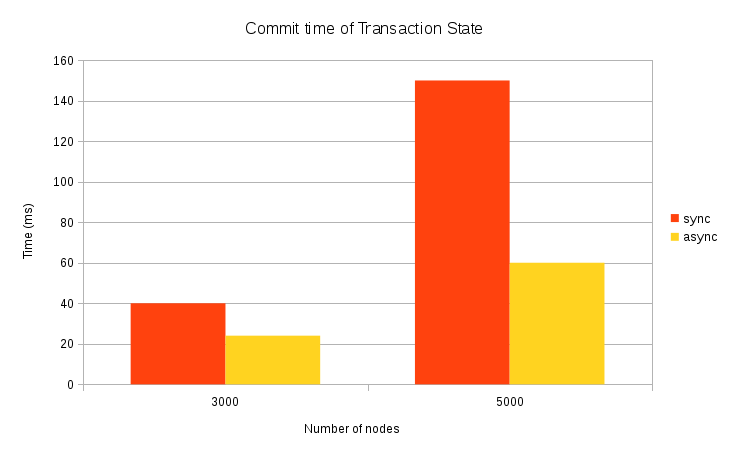
\includegraphics[scale=0.7]{resources/images/Evaluation/ts_commit_sync_async.png}
\caption{TS commit time with GC service}
\label{fig:ev_ts_sync_async}
\end{figure}

In Figure \ref{fig:ev_ts_sync_async} is depicted the total time taken
in milliseconds to persist the TS for 3000 and 5000 nodes in the
cluster. The time to commit affects both the scheduler and the
ResourceTracker regarding the updated view of the cluster and this has
a direct impact on the cluster utilization. For the simulation with
3000 NodeManagers the average commit time, even though it was already
low it dropped 24 ms from 40 ms. The difference is more visible
for the simulation with 5000 nodes in the cluster where the commit
time dropped to 60 ms from 150 ms. In general we can observe a tension
to half the commit time and this is reasonable for several
reasons. First and foremost is because we do not have the foreign key
constraints in the tables that store RPCs (Figure
\ref{fig:impl_fk_yarn_rpc}). Also, the removal of old values is done
asynchronously so no overhead in the commit phase of the TS. Finally,
we have removed some \texttt{flush} operations from the application
logic that had to be there before to serialize the queries.


\begin{figure}
\centering
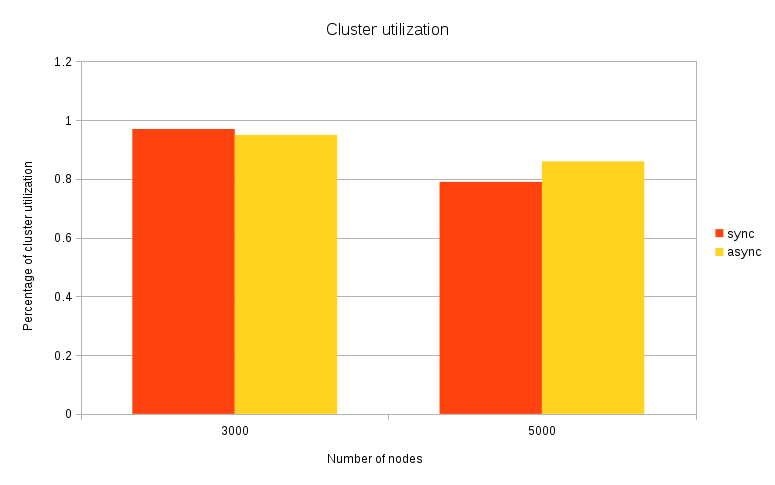
\includegraphics[scale=0.7]{resources/images/Evaluation/cluster_util_sync_async.png}
\caption{Cluster utilization with GC service}
\label{fig:ev_cluster_util_sync_async}
\end{figure}

The improvements on the commit time had a direct impact also in the
cluster utilization as we can see in Figure
\ref{fig:ev_cluster_util_sync_async}. For a 3000 nodes cluster the
utilization remained almost the same but it was already high
enough. Nevertheless, we have managed to improve the cluster
utilization by a few percentages for a 5000 nodes simulation, reaching
86 $\%$. The number of containers created in a 5000 nodes cluster
increased by 10$\%$ with the Garbage Collector service while in a 3000
nodes cluster it remained almost the same. Moreover, there is interesting
side effect with decreased commit time. Since, TSs take less time to
commit, the blocking TSs that cannot be aggregated also spent less
time in the waiting queues of the Transaction Manager. That leads to
``smaller'' but more AggregatedTransactionStates. For instance, in the
simulation with 5000 NodeManagers without the GC service, there were
roughly 900 TS commits with on average 2000 objects to persist just
to update the status of NodeManagers. On the contrary, with the GC
service, there were 1690 TS commits with 960 objects to persist for
the NodeManagers. This side effect also helped vanish the rollback of
transactions due to overloading (Section \ref{sssec:impl_aggr_new}), 
since there were not that many TSs in the queue to aggregate.

\section{DTO caching}
\label{sec:ev_dto_caching}
In Section \ref{sec:dto_caching} the issue of
creating Data Transfer Objects with ClusterJ was introduced. In Figure
\ref{fig:impl_dto_no_cache} is depicted the time needed to create a number of
DTOs and persist them in the database. The evaluation of the Caching
mechanism was done both with a micro-benchmark but also with simulations
measuring the time to commit a Transaction State in the database,
the cluster utilization and also the number of heartbeats that the
scheduler is processing. The simulations were performed in the second
type of setup.

\begin{figure}
\centering
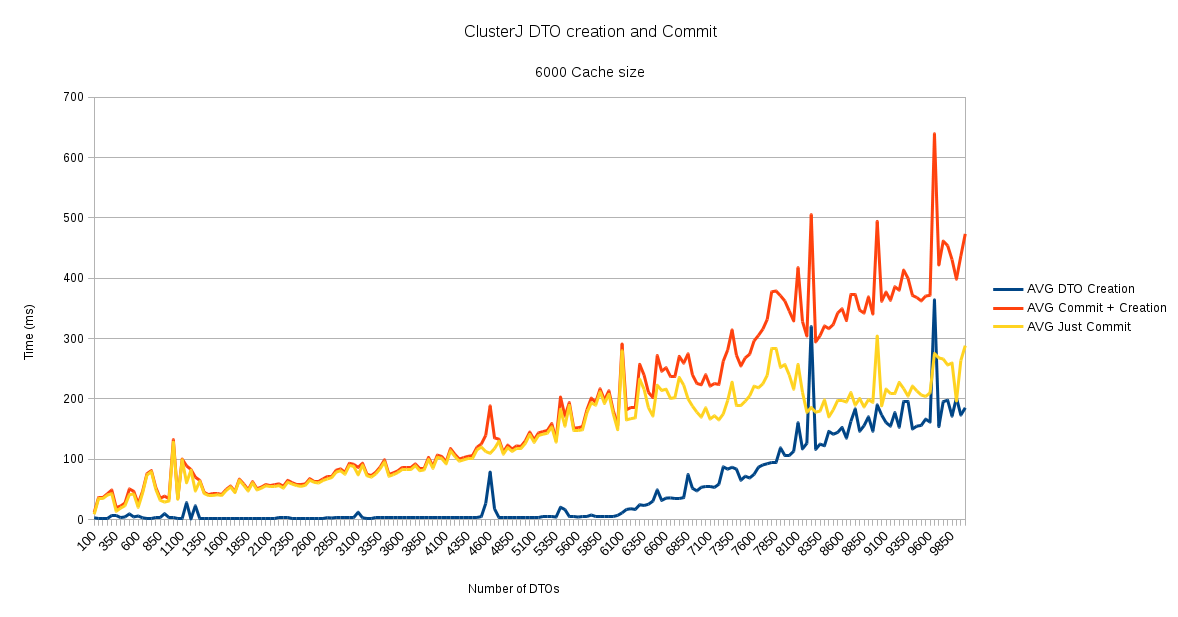
\includegraphics[scale=0.5]{resources/images/Evaluation/dto_creation_cache_bench.png}
\caption{DTO creation and commit with cache enabled}
\label{fig:ev_dto_creation_bench}
\end{figure}

In Figure \ref{fig:ev_dto_creation_bench} is the result of the same
micro-benchmark performed in Section \ref{sec:dto_caching} but with
the Caching mechanism. The blue line is the creation time of DTOs, the
yellow line is the actual commit time and the red one is both the
creation and the commit time. The cache size of the sessions was 6000
objects. Comparing the two figures, the difference in the creation
time is massive. The ``creation'' time in the second case is almost
zero until the cache limit is reached. Even when the number of DTOs
requested are more than the cache size, it is still much faster. At
the time the benchmark was done, the cache size of the sessions was
fixed to a number. It is expected the performance to be better with the
dynamic size of the cache.

The next evaluation parameter is the mean time for a Transaction State
to be committed in the database. The parameters of the cache are
outlined in Table \ref{tab:ev_cache_conf}. It is not possible to cache
all the DTO types mainly for two reasons. First, it would take more
time to fill-up the cache with more types which would result in
very few \emph{ready} sessions. So the transactions would use
non-cached sessions or even worse fall-back to creating new
sessions. The second reason is memory related. Even though DTOs are
not allocated on the heap of the JVM and do not account to Java
garbage collection, they still consume memory from the machine that
could be used for scheduling decisions or handling of heartbeats. In
Figure \ref{fig:ev_cache_ts_commit} is the average commit time of a
TransactionState object with cache-enabled and cache-disabled
sessions. Even with a cluster size of 2000 nodes there is a small
difference in the commit time. As the number of NodeManagers grows,
the difference is getting wider reaching almost 20 ms in 10000 nodes
cluster.

\begin{table}
\centering
\begin{tabular}{| c | c | c | c |}
\hline
\textbf{Type} & \textbf{Min. size} & \textbf{Max. size} & \textbf{Step}\\
\hline
\hline
PendingEventDTO & 12000 & 25000 & 400\\
\hline
NodeHBResponseDTO & 2000 & 10000 & 200\\
\hline
UpdatedContainerInfoDTO & 2000 & 10000 & 200\\
\hline
\end{tabular}
\caption{Cache mechanism configuration}
\label{tab:ev_cache_conf}
\end{table}

\begin{figure}
\centering
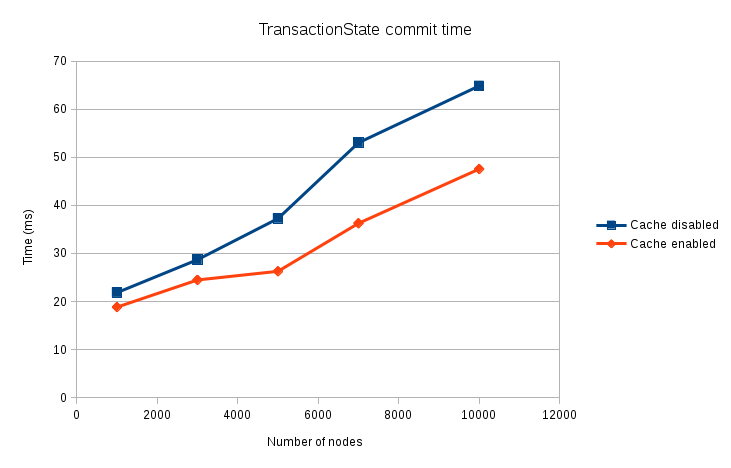
\includegraphics[scale=0.6]{resources/images/Evaluation/dto_cache_ts_commit.png}
\caption{TS commit time with and without cache}
\label{fig:ev_cache_ts_commit}
\end{figure}

\begin{figure}
\centering
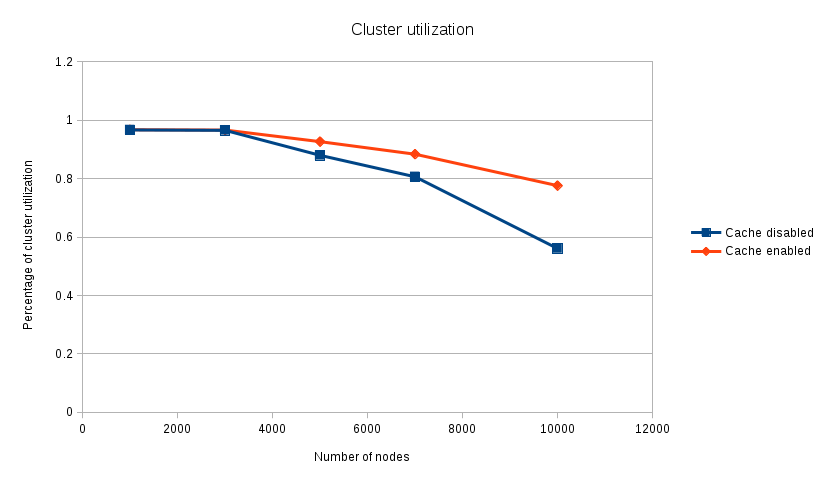
\includegraphics[scale=0.6]{resources/images/Evaluation/dto_cache_cluster_util.png}
\caption{Cluster utilization with and without cache}
\label{fig:ev_cache_cluster_util}
\end{figure}

The improvement in the commit time is reflected in the cluster
utilization as illustrated in Figure \ref{fig:ev_cache_cluster_util}.
Until 3000 nodes there is no difference in the utilization but the more
NodeManagers in the simulation, the bigger is the difference. In 10000
nodes simulation the cluster utilization increased from 56$\%$ to
77$\%$ and the launched containers from 167177 to 247032 (Figure
\ref{fig:ev_cache_containers}).

\begin{figure}
\centering
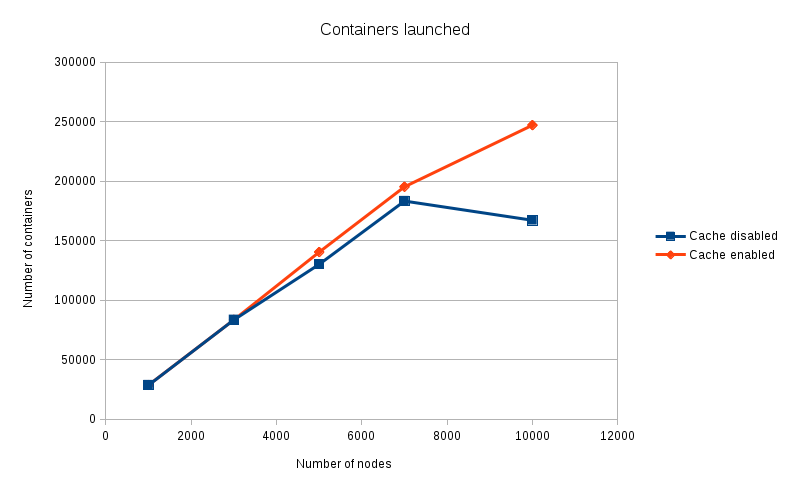
\includegraphics[scale=0.6]{resources/images/Evaluation/dto_cache_containers.png}
\caption{Containers launched with and without cache}
\label{fig:ev_cache_containers}
\end{figure}

\begin{figure}
\centering
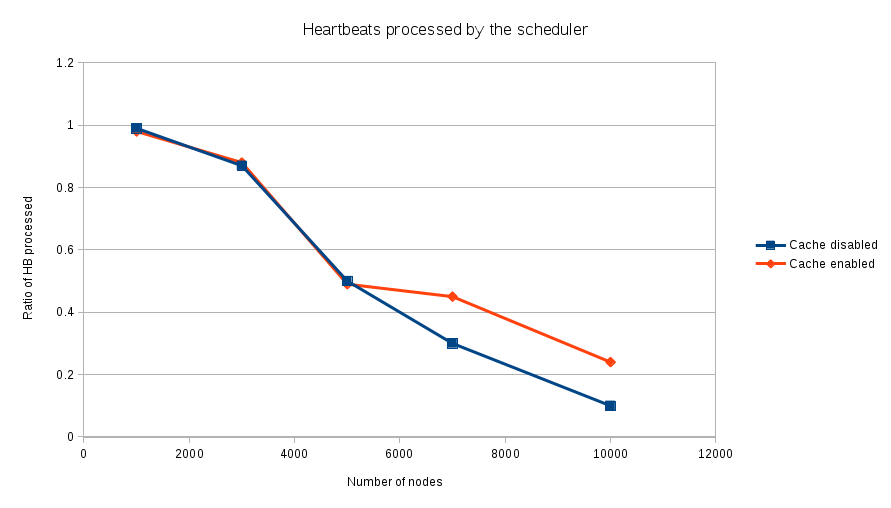
\includegraphics[scale=0.6]{resources/images/Evaluation/dto_cache_hb_processed.png}
\caption{HB processed with and without cache}
\label{fig:ev_cache_hb_processed}
\end{figure}

Finally, the number of heartbeats processed by the scheduler node has
also been increased but  still is quite low
affecting the scheduling decisions. In Figure
\ref{fig:ev_cache_hb_processed} is depicted the ratio of
heartbeats processed by the RM over the total number of
heartbeats. For a 10000 nodes cluster the ratio is still very low but
until 5000 NodeManagers is quite acceptable.

\section{Performance overview}
\label{sec:performance_overview}
Until now we have presented the improvements in performance that each
step of the implementation has contributed. In order to verify that
the goals of this project have been achieved a comparison should be
made between the latest version of the Hops-YARN with the version
before the thesis. Also, since Hops-YARN is a fork of Apache YARN, the
big question is how our implementation performs in comparison with the
upstream YARN in terms of cluster utilization. In Figure \ref{fig:ev_cluster_util_final} is depicted
the cluster utilization for various number of nodes in a cluster. 
The yellow line is the \texttt{develop} branch of Hops-YARN, the code
base before this thesis. The blue line is the
\texttt{merge\_tx\_no\_fk} branch which is the final version of this
thesis and the red line is Apache Hadoop 2.4.0 There are two observations
that should be noticed in this figure. The first one is the
improvement over the \texttt{develop} branch. Already from 3000 nodes
we can notice a small difference. Starting from 3000 nodes,
the cluster utilization of the \texttt{develop} branch drops very
roughly until 10000 nodes where it is 35$\%$. With the modifications
proposed in this thesis the cluster utilization curve is more flat
with an acceptable rate for the whole range of simulations.

\begin{figure}
\centering
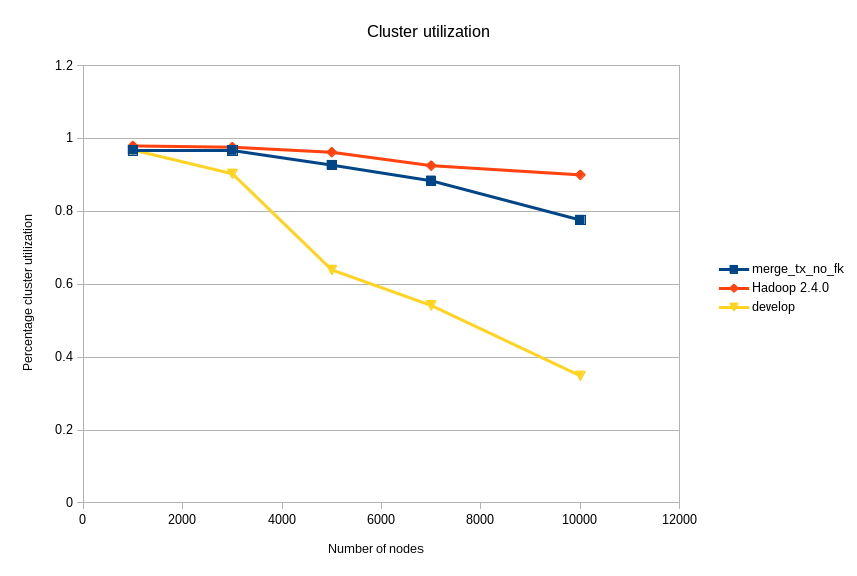
\includegraphics[scale=0.6]{resources/images/Evaluation/cluster_usage_final.png}
\caption{Cluster utilization comparison, Hops-YARN - Apache YARN}
\label{fig:ev_cluster_util_final}
\end{figure}

The second observation is the gap between \texttt{merge\_tx\_no\_fk} and
Hadoop 2.4.0 Until 7000 NodeManagers the difference is very small,
88$\%$ and 92$\%$ respectively. Even with the largest configuration
of 10000 nodes the difference is 13$\%$ in cluster utilization which
is not negligible but considering the lower recovery time of Hops-YARN
and the distributed ResourceManagers it might be a valid trade-off.

The next evaluation parameter for the project is the ratio of
heartbeats processed by the scheduler over the total number of
heartbeats. Hops-YARN has distributed the ResourceTrackerService which
receives heartbeats from NodeManagers, persists the information
received in NDB and then it is streamed to the master ResourceManager
which updates its view of the cluster. In Figure
\ref{fig:ev_hb_processed_final} is illustrated the heartbeat ratio for
the \texttt{develop} and \texttt{merge\_tx\_no\_fk} branch and Hadoop
2.4.0 We can observe a great improvement up until 4000
NodeManagers. Although the difference is small for the rest of the
simulations, it is constantly better than in \texttt{develop} branch
of Hops-YARN. Apache Hadoop never drops below 94$\%$ but it is
necessary to
mention that Apache YARN is a centralized architecture with no
communication latency between the ResourceTrackerService and the scheduler.

\begin{figure}
\centering
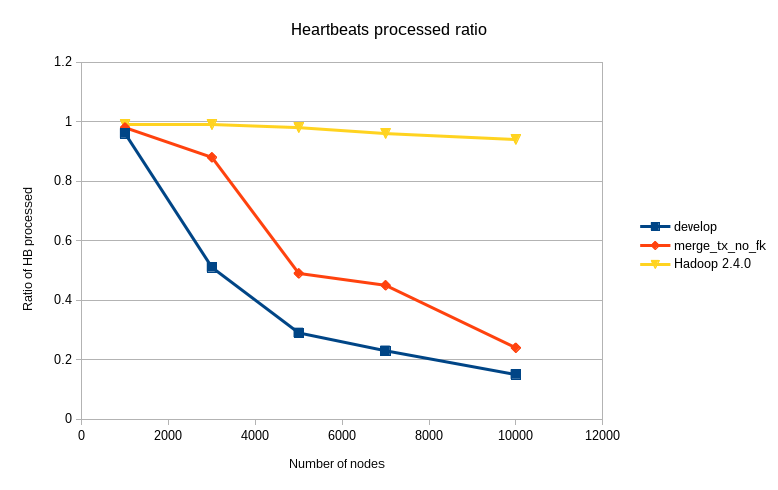
\includegraphics[scale=0.7]{resources/images/Evaluation/hb_processed_final.png}
\caption{Ratio of processed heartbeats}
\label{fig:ev_hb_processed_final}
\end{figure}

Finally, for the completeness of the evaluation it is worth to mention the
CPU utilization and memory
consumption (Figure  \ref{fig:ev_cpu_util_rm_rt}, \ref{fig:ev_mem_consumption_rm_rt}) of the
ResourceManager -- \textbf{bbc7} and the
ResourceTracker -- \textbf{bbc6}. Throughout the simulation with 10000 nodes in a
cluster, the average CPU usage of RM never went above 20$\%$ while for
the RT the maximum average is 45$\%$. Regarding the memory consumption
for the same simulation, both RM and RT never used more than 24GB of RAM.

\begin{figure}
\centering
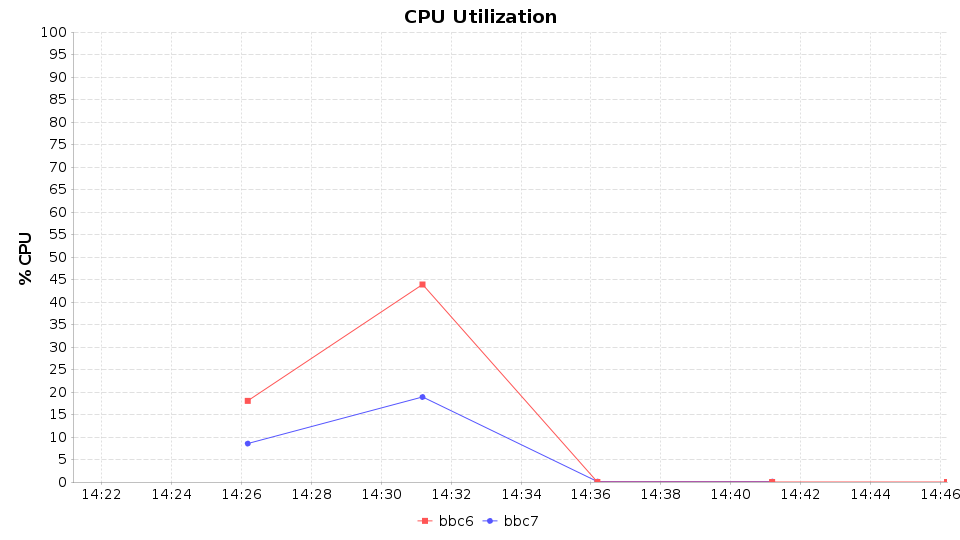
\includegraphics[scale=0.4]{resources/images/Evaluation/RM_RT_cpu_utilization.png}
\caption{CPU usage for RM (bbc7) and RT (bbc6)}
\label{fig:ev_cpu_util_rm_rt}
\end{figure}

\begin{figure}
\centering
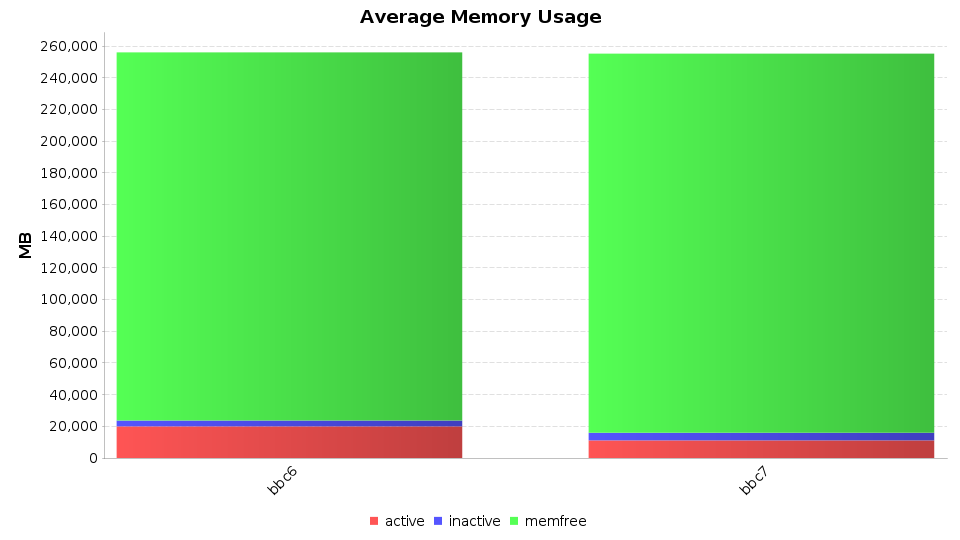
\includegraphics[scale=0.4]{resources/images/Evaluation/RM_RT_memory_usage.png}
\caption{Memory usage for RM (bbc7) and RT (bbc6)}
\label{fig:ev_mem_consumption_rm_rt}
\end{figure}


\chapter{Conclusions}
\label{chap:conclusion}

\section{Conclusion}
\label{sec:conclusion}
In Hops-YARN, as it is already mentioned, MySQL Cluster NDB is used
both as a communication transport and as a persistent storage for
recovery. At the beginning of the project a thorough profiling of the
execution workflow has been done to identify the bottlenecks of the
system. The first step was to remove the foreign key constraints from
the database schema used by Hops-YARN. In Section
\ref{sec:fk_constraints} is explained how they were replaced by
application logic that performs primary key operations. Section
\ref{sec:tx_aggregation} discusses the evolution of the commit
mechanism which squashes several blocked transaction into a ``big''
one reducing the number of commits in the back-end database
system. Section \ref{sec:gc_service} presents the Garbage Collector
service of Hops-YARN that removes asynchronously old values from the
database. With that solution the commit time dropped more improving
the overall performance of the system. Finally, Section
\ref{sec:dto_caching} explains how the shortcoming of ClusterJ for
creating DTOs was bypassed by having created them ahead of time in a
per session cache.

After a detailed explanation of the solutions proposed, in Chapter
\ref{chap:evaluation} follows the evaluation. Each solution is
evaluated separately by simulating real world traces. In each case key
characteristics are examined and how they have been improved. In
Section \ref{sec:performance_overview} there is an overall performance
overview in terms of cluster utilization and heartbeats processed by
the scheduler. The comparison is made among the version of Hops-YARN
before this project, the final version with all the modification
proposed and the upstream Apache YARN. The figures show that there was
a clear improvement, in both evaluation parameters, when the two
version of Hops-YARN are compared. Finally, as far as the cluster
utilization is concerned, the performance is comparable with Apache
YARN in clusters with thousands of nodes.

\subsection{Goals}
\label{ssec:goals}
In Chapter \ref{chap:introduction} the goals of this project were
set. The primary goals was to improve the cluster utilization and the
number of heartbeats processed by the scheduler. In order to achieve
those goals we have also set some sub-goals. With the solutions proposed
in Chapter \ref{chap:implementation} all the sub-goals were met. In
particular, with the removal of the foreign key constraints and the
DTO caching mechanism the transactional commit time was decreased
dramatically. Some sort of asynchronous API was provided by the
garbage collector service. It is provided only for a small sub-set but
still it made big difference to the performance of the system. The new
aggregation mechanism of the transaction manager of Hops-YARN helped
the blocked transactions to be committed faster which in turn improved the
parallelization of the system. Finally, in each step of the
implementation an evaluation was done to prove the performance impact
and guide us to new bottlenecks.

Since all the sub-goals were met it was expected to achieve the
primary goals. As Chapter \ref{chap:evaluation} indicates the two
primary goals were also accomplished. Both cluster utilization and the
heartbeat ratio was improved.


\subsection{Insights and suggestions for further work}
\label{ssec:insights-and-suggestions}
This is the insights section

\section{Future work}
\label{sec:future-work}
A few things have been left undone due to time limitation and are
discussed in this section for future work.

In most of the cases the evaluation has been done using simulations
measuring among others the cluster utilization while in others the
evaluation has been done using benchmarks. It would be more complete
if in all cases the benchmarks were supported by simulation
results. That way the performance improvements introduced by each step
would be more clear.

Currently we do not have any insight on the content of Transaction
State objects, thus they are treated equally. In real world scenarios,
during the allocation of resources, the Transaction State would carry
more information about allocated containers than when the cluster is
full and no further allocations can be made. A fine-grained inspection
on the content of a TS might improve performance further more. For
example in the commit mechanism, when an Aggregated Transaction State
object is overloading NDB, the transaction will roll-back and the
aggregation policy will enforce a lower limit. If we had any
information on the content of the TS before hand, this situation could
have been avoided.

As it is already mentioned, the Garbage Collector service does not
perform primary key operations. It was a design decision that would
not complicate the mechanism and burden the commit time by committing
more information. It is worth trying to persist all the columns needed
for the primary keys to be reconstructed and measure the
performance. For sure the deletion time would be lower but it
remains to be proven if that will have any impact on the performance
of Hops-YARN in general.

Last but not least, the batching system explained in Section
\ref{ssec:impl_batch_system} should be improved. Changing the number
of RPCs that are batched together did not change the
performance. Every RPC arriving in the ResourceManager among others it
should get the current Transaction State object from the Transaction State
Manager. This operation could take $0.06$ ms. If we consider a cluster
with 10000 NodeManagers heartbeating every second, it is needed 600 ms
just to acquire the object. At the time of writing that was the latest
bottleneck encountered and for sure it is worth for future investigation.

\subsection{What has been left undone?}
\label{ssec:what-has-been-left-undone}
This is what has been left undone


%%\bibliography{report}
%%\bibliographystyle{IEEEtran}
%%\bibliographystyle{unsrturl}
%%\bibliographystyle{unsrtnat}
%%\bibliographystyle{myIEEEtran}

\printbibliography[heading=bibintoc]

\appendix
\chapter{Insensible Approximation}

\backmatter

\end{document}
